\documentclass{tufte-book}

\hypersetup{colorlinks}% uncomment this line if you prefer colored hyperlinks (e.g., for onscreen viewing)

%%
% Book metadata
\title{The BlackBook}
\author[The Black family]{The Black family}
\publisher{The Black family recipe book, typeset in \LaTeX by James}

%%
% If they're installed, use Bergamo and Chantilly from www.fontsite.com.
% They're clones of Bembo and Gill Sans, respectively.
%\IfFileExists{bergamo.sty}{\usepackage[osf]{bergamo}}{}% Bembo
%\IfFileExists{chantill.sty}{\usepackage{chantill}}{}% Gill Sans

%\usepackage{microtype}

%%
% Just some sample text
\usepackage{lipsum}

%%
% For nicely typeset tabular material
\usepackage{booktabs}


%%
% For graphics / images
\usepackage{graphicx}
\setkeys{Gin}{width=\linewidth,totalheight=\textheight,keepaspectratio}
\graphicspath{{graphics/}}

% The fancyvrb package lets us customize the formatting of verbatim
% environments.  We use a slightly smaller font.
\usepackage{fancyvrb}
\fvset{fontsize=\normalsize}

%%
% Prints argument within hanging parentheses (i.e., parentheses that take
% up no horizontal space).  Useful in tabular environments.
\newcommand{\hangp}[1]{\makebox[0pt][r]{(}#1\makebox[0pt][l]{)}}

%%
% Prints an asterisk that takes up no horizontal space.
% Useful in tabular environments.
\newcommand{\hangstar}{\makebox[0pt][l]{*}}

%%
% Prints a trailing space in a smart way.
\usepackage{xspace}

%%
% Some shortcuts for Tufte's book titles.  The lowercase commands will
% produce the initials of the book title in italics.  The all-caps commands
% will print out the full title of the book in italics.
\newcommand{\vdqi}{\textit{VDQI}\xspace}
\newcommand{\ei}{\textit{EI}\xspace}
\newcommand{\ve}{\textit{VE}\xspace}
\newcommand{\be}{\textit{BE}\xspace}
\newcommand{\VDQI}{\textit{The Visual Display of Quantitative Information}\xspace}
\newcommand{\EI}{\textit{Envisioning Information}\xspace}
\newcommand{\VE}{\textit{Visual Explanations}\xspace}
\newcommand{\BE}{\textit{Beautiful Evidence}\xspace}

\newcommand{\TL}{Tufte-\LaTeX\xspace}

% Prints the month name (e.g., January) and the year (e.g., 2008)
\newcommand{\monthyear}{%
  \ifcase\month\or January\or February\or March\or April\or May\or June\or
  July\or August\or September\or October\or November\or
  December\fi\space\number\year
}


% Prints an epigraph and speaker in sans serif, all-caps type.
\newcommand{\openepigraph}[2]{%
  %\sffamily\fontsize{14}{16}\selectfont
  \begin{fullwidth}
  \sffamily\large
  \begin{doublespace}
  \noindent\allcaps{#1}\\% epigraph
  \noindent\allcaps{#2}% author
  \end{doublespace}
  \end{fullwidth}
}

% Inserts a blank page
\newcommand{\blankpage}{\newpage\hbox{}\thispagestyle{empty}\newpage}

\usepackage{units}

% Typesets the font size, leading, and measure in the form of 10/12x26 pc.
\newcommand{\measure}[3]{#1/#2$\times$\unit[#3]{pc}}

% Macros for typesetting the documentation
\newcommand{\hlred}[1]{\textcolor{Maroon}{#1}}% prints in red
\newcommand{\hangleft}[1]{\makebox[0pt][r]{#1}}
\newcommand{\hairsp}{\hspace{1pt}}% hair space
\newcommand{\hquad}{\hskip0.5em\relax}% half quad space
\newcommand{\TODO}{\textcolor{red}{\bf TODO!}\xspace}
\newcommand{\ie}{\textit{i.\hairsp{}e.}\xspace}
\newcommand{\eg}{\textit{e.\hairsp{}g.}\xspace}
\newcommand{\na}{\quad--}% used in tables for N/A cells
\providecommand{\XeLaTeX}{X\lower.5ex\hbox{\kern-0.15em\reflectbox{E}}\kern-0.1em\LaTeX}
\newcommand{\tXeLaTeX}{\XeLaTeX\index{XeLaTeX@\protect\XeLaTeX}}
% \index{\texttt{\textbackslash xyz}@\hangleft{\texttt{\textbackslash}}\texttt{xyz}}
\newcommand{\tuftebs}{\symbol{'134}}% a backslash in tt type in OT1/T1
\newcommand{\doccmdnoindex}[2][]{\texttt{\tuftebs#2}}% command name -- adds backslash automatically (and doesn't add cmd to the index)
\newcommand{\doccmddef}[2][]{%
  \hlred{\texttt{\tuftebs#2}}\label{cmd:#2}%
  \ifthenelse{\isempty{#1}}%
    {% add the command to the index
      \index{#2 command@\protect\hangleft{\texttt{\tuftebs}}\texttt{#2}}% command name
    }%
    {% add the command and package to the index
      \index{#2 command@\protect\hangleft{\texttt{\tuftebs}}\texttt{#2} (\texttt{#1} package)}% command name
      \index{#1 package@\texttt{#1} package}\index{packages!#1@\texttt{#1}}% package name
    }%
}% command name -- adds backslash automatically
\newcommand{\doccmd}[2][]{%
  \texttt{\tuftebs#2}%
  \ifthenelse{\isempty{#1}}%
    {% add the command to the index
      \index{#2 command@\protect\hangleft{\texttt{\tuftebs}}\texttt{#2}}% command name
    }%
    {% add the command and package to the index
      \index{#2 command@\protect\hangleft{\texttt{\tuftebs}}\texttt{#2} (\texttt{#1} package)}% command name
      \index{#1 package@\texttt{#1} package}\index{packages!#1@\texttt{#1}}% package name
    }%
}% command name -- adds backslash automatically
\newcommand{\docopt}[1]{\ensuremath{\langle}\textrm{\textit{#1}}\ensuremath{\rangle}}% optional command argument
\newcommand{\docarg}[1]{\textrm{\textit{#1}}}% (required) command argument
\newenvironment{docspec}{\begin{quotation}\ttfamily\parskip0pt\parindent0pt\ignorespaces}{\end{quotation}}% command specification environment
\newcommand{\docenv}[1]{\texttt{#1}\index{#1 environment@\texttt{#1} environment}\index{environments!#1@\texttt{#1}}}% environment name
\newcommand{\docenvdef}[1]{\hlred{\texttt{#1}}\label{env:#1}\index{#1 environment@\texttt{#1} environment}\index{environments!#1@\texttt{#1}}}% environment name
\newcommand{\docpkg}[1]{\texttt{#1}\index{#1 package@\texttt{#1} package}\index{packages!#1@\texttt{#1}}}% package name
\newcommand{\doccls}[1]{\texttt{#1}}% document class name
\newcommand{\docclsopt}[1]{\texttt{#1}\index{#1 class option@\texttt{#1} class option}\index{class options!#1@\texttt{#1}}}% document class option name
\newcommand{\docclsoptdef}[1]{\hlred{\texttt{#1}}\label{clsopt:#1}\index{#1 class option@\texttt{#1} class option}\index{class options!#1@\texttt{#1}}}% document class option name defined
\newcommand{\docmsg}[2]{\bigskip\begin{fullwidth}\noindent\ttfamily#1\end{fullwidth}\medskip\par\noindent#2}
\newcommand{\docfilehook}[2]{\texttt{#1}\index{file hooks!#2}\index{#1@\texttt{#1}}}
\newcommand{\doccounter}[1]{\texttt{#1}\index{#1 counter@\texttt{#1} counter}}

% Generates the index
%\usepackage{makeidx}
\usepackage[makeindex, split]{splitidx}

\makeindex
\newindex[Recipes]{recipe}

\usepackage{ gensymb } % for celcius

\geometry{height=10.250in,width=8.125in}

\begin{document}

% Front matter
\frontmatter

% r.1 blank page
%\blankpage

% r.3 full title page
\maketitle


% v.4 copyright page
\newpage
\begin{fullwidth}
~\vfill
\thispagestyle{empty}
\setlength{\parindent}{0pt}
\setlength{\parskip}{\baselineskip}
Copyright \copyright\ \the\year\ \thanklessauthor

\par\smallcaps{This is \thanklesspublisher}

\par\smallcaps{The tastiest recipes, all vetted by Tina and James}

\par The majority of these recipes are from Bill's recipe notebook, which is a continuous document that he has curated over many years. He makes no claim to inventing the recipe, but every recipe has been meticulously tested. This book is designed to be written in, and updated. Much like the original notebook this recipe book is based on. Unless required by applicable law or agreed to in writing, recipes distributed here are on a \smallcaps{``AS IS'' BASIS, WITHOUT WARRANTIES OR CONDITIONS OF ANY KIND}, either express or implied. We take no responsibility for any kitchen disasters that you may experience.

\par\textit{A continuous document, last compiled \monthyear}
\end{fullwidth}

% v.2 epigraphs
\newpage\thispagestyle{empty}
\openepigraph{%
Is there that owre his French ragout,
Or olio that wad staw a sow,
Or fricassee wad mak her spew
Wi perfect scunner,
Looks down wi sneering, scornfu view
On sic a dinner?
}{Robbie Burns, \emph{Address to a Haggis}%, {\itshape Design, Form, and Chaos}
}
\vfill
\openepigraph{%
After a good dinner one can forgive anybody, even one's own relations.
}{Oscar Wilde, \emph{A Woman of No Importance}}
\vfill
\openepigraph{%
Let food be thy medicine and medicine be thy food.
}{Hippocrates}
\vfill
\openepigraph{%
Training is everything. The peach was once a bitter almond;\break cauliflower is nothing but cabbage with a college education.
}{Mark Twain}
\vfill
\openepigraph{%
Vegetarians, and their Hezbollah-like splinter faction, the vegans ... are the enemy of everything good and decent in the human spirit.
}{Anthony Bourdain, \emph{Kitchen Confidential}}

% r.5 contents
\cleardoublepage
\tableofcontents

%\listoffigures
%\listoftables

% r.7 dedication
\cleardoublepage
~\vfill
\begin{doublespace}
\noindent\fontsize{16}{18}\selectfont\itshape
\nohyphenation
Dedicated to Nana, Bill and Dama 

for all the awesome food they introduced me to.
\end{doublespace}
\vfill
\vfill




%%
% Start the main matter (normal chapters)
\mainmatter

%example four pictures
\begin{figure*}[p]
\fbox{\includegraphics[width=0.45\linewidth,height=0.45\textheight]{graphics/breadcrumb_cover.png}}
\hfill
\fbox{\includegraphics[width=0.45\linewidth,height=0.45\textheight]{graphics/blackpuddingragout_cover.JPG}}
\\\vspace{\baselineskip}
\fbox{\includegraphics[width=0.45\linewidth,height=0.45\textheight]{graphics/pearsaladabove_cover.JPG}}
\hfill
\fbox{\includegraphics[width=0.45\linewidth,height=0.45\textheight]{graphics/bossam_cover.png}}
\end{figure*}

%%%%%%%%%%%%%%%%%%%%%%%%%%%%%%%%%%%%%%%%%
\chapter{Brunch}
%%%%%%%%%%%%%%%%%%%%%%%%%%%%%%%%%%%%%%%%%

\begin{figure*}[h]
  \includegraphics[width=\linewidth]{tacobell.jpg}
\end{figure*}

\section{Breakfast burritos}
\index{Brunch!burritos}

While the photo above is a Taco Bell double cheese and beef burrito, it summarises the point of breakfast burritos. They are an offensively American invention, that is a worthwhile extravagance that will sooth the morning after a big night out.

Cheesy eggs and tortillas are the only essentials here. It's also nice to add some starch, salsa and avocado. If you have the time, beans cooked with browned onions and minced chorizo, then lightly mashed makes an amazing refried beans.

\smallskip
\emph{Cheesy scrambled eggs
\\Tortillas
\\Chorizo or sausage
\\Avocado/tomato/baby spinach
\\Refried beans
\\Hashbrowns/bratkartoffeln
}

\begin{marginfigure}%
  \includegraphics[width=\linewidth]{burrito.jpg}
\end{marginfigure}

\smallskip
Pick the elements you want and roll! Super cheesy scrambled eggs is essential if you don't have salsa.

%%%%%%%%%%%%%%%%%%%%%%%%%%%%%%%%%%%%%%%%%
\newpage

\begin{figure*}[h]
  \includegraphics[width=\linewidth]{turkisheggs.png}
\end{figure*}

\section{Turkish eggs}
\index{Brunch!Turkish eggs}

My favourite brunch dish is from \emph{Kopapa} in London, where I had the Turkish eggs one morning with Dad. Two poached eggs on a bed of garlicky yoghurt swimming in spiced melted butter. Amazingly good with some good crusty bread for dipping. The recipe is for one. 

\smallskip
\emph{2 eggs
\\1/2 cup greek yogurt
\\1 clove garlic, minced
\\1 tsp paprika
\\1/2 tbsp butter
\\Dried mint flakes
\\Optional: Fresh or dried chilli
}

\smallskip
Start poaching the eggs.
\\Melt the butter in a pan with the paprika, when it foams or browns, take off the heat. Season with salt and pepper. If adding chillies, add them to this butter mix.
\\Whip the minced garlic into the yogurt. Season.
\\Once the eggs are poached, place on top of the yoghurt in a bowl.
\\Pour the butter on top, serve with bread.

%%%%%%%%%%%%%%%%%%%%%%%%%%%%%%%%%%%%%%%%%
\newpage

\begin{figure*}[h]
  \includegraphics[width=\linewidth]{kedgeree2.JPG}
\end{figure*}

\section{Kedgeree}
\index{Seafood curry!seafood}
\index{Brunch!kedgeree}
\index{Rice!kedgeree}

Not the usual brunch fare, but this colonial throwback can also make an easy dinner. Recipe serves two.

\smallskip
\newpart{For the rice:}
\\\emph{120g rice
\\600ml stock
\\2 eggs
\\1 onion sliced
\\3 cloves garlic
\\1 tbsp English curry powder
\\1 tsp tumeric
\\5 curry leaves or 3 bay leaves
\\2 fillets smoked fish\sidenote{
In the photo we also added some cooked seafood right before serving.}
\\1 chilli
\\1 tbsp butter
\\1 lemon sliced into quarters
}

\newpage

\newpart{For the yoghurt:}
\\\emph{Big handful coriander finely cut
\\1/2 cup yoghurt
\\Zest of 1 lemon
}

\begin{marginfigure}%
  \includegraphics[width=\linewidth]{kedgeree.png}
\end{marginfigure}

\smallskip
Get 600ml of stock to the boil, then add the eggs and set the timer to soft boiled (take eggs out of the stock when they are cooked).
\\In another pan, fry the onion with the curry powder, tumeric and a little oil. After a few minutes, add the garlic.
\\Once the onion is starting to brown, add the rice and stir. As soon as it's mixed, add in the stock. 
\\Keep the rice on medium high and occasionally stir. You might need to add a little water.
\\Once the rice is cooked, add in the seafood and butter. Season after tasting, as the fish might be salty. Serve with lemon wedges and sprinkle coriander on as garnish.
\\Mix the yoghurt, lemon rind and coriander. Serve with rice.

%%%%%%%%%%%%%%%%%%%%%%%%%%%%%%%%%%%%%%%%%

\section{Crisp omelette}
\index{Brunch!crisp omelette}

This recipe is from Ferrian Adria's \emph{"kitchen meal"} cookbook. The recipe is for two as a light meal. Strange to see chips in a Michelin starred chefs cookbook.. but it actually works.

\smallskip
\emph{4 tbsp olive oil
\\6 eggs
\\70g salted potato chips
}

\smallskip
Break the eggs into a bowl and whip till frothy.
\\Add the chips and lightly mix, then leave for one minute.
\\Add half the oil to the pan and cook egg mixture for 40 seconds.
\\Once the top has set, flip onto a plate then add the last half of the oil and slide the omelette back into the pan and cook for a final 20 seconds.

%%%%%%%%%%%%%%%%%%%%%%%%%%%%%%%%%%%%%%%%%
\newpage

\begin{figure*}[h]
  \includegraphics[width=\linewidth]{aspandeggs.png}
\end{figure*}

\section{Asparagus, mushroom, eggs \& garlic crumbs}
\index{Brunch!asparagus, mushroom and eggs}

A super easy summer dish. Can also be eaten for dinner. The asparagus and mushrooms can be cooked earlier, and then lightly reheated. 

\smallskip
\emph{2 tbsp olive oil
\\4 eggs
\\4 portobello mushrooms
\\2 handfuls asparagus
\\2 tbsp butter
\\1 clove minced garlic
\\1 anchovy fillet minced
\\Dash Worcester sauce
}

\smallskip
Trim the mushrooms, drizzle with oil, season and fry till brown.
\\Poach the eggs.
\\Drop the asparagus into the egg poaching water for 2 minutes.
\\Add the butter,  garlic and anchovy to a pan and fry till both the garlic and the butter are a deep brown. At the last minute, flick some  Worcester sauce into the butter and mix.
\\Plate the asparagus, mushrooms and eggs then drip over garlic crumbs.

%%%%%%%%%%%%%%%%%%%%%%%%%%%%%%%%%%%%%%%%%
\newpage

\begin{figure*}[h]
  \includegraphics[width=\linewidth]{potatoscones.png}
\end{figure*}

\section{Potato scones}
\index{Brunch!potato scones}
\index{Potato!scones}

An easy and tasty meal. Keep well in the refrigerator for several days. 

\begin{marginfigure}%
  \includegraphics[width=\linewidth]{potatoscones_meal.png}
\end{marginfigure}

\smallskip
\emph{225g boiled and mashed potatoes
\\65g flour 
\\3 tbsp melted butter
\\Half tsp salt
\\$\frac{1}{4}$ tsp of baking powder
}

\smallskip
Mash the potatoes while they are still warm and add the butter and salt. 
\\Add in enough flour to make it a pliable dough but without making it too dry. The type of potato will affect this. 
\\Turn out onto a floured surface and roll until about quarter of an inch thick. Cut into six inch circles and then into quarters. 
\\Prick all over with a fork and cook in a heavy pan which has been lightly greased with butter. 
\\Cook each side for about three minutes or until golden brown.

%%%%%%%%%%%%%%%%%%%%%%%%%%%%%%%%%%%%%%%%%
\newpage

\section{Plum cake}
\index{Brunch!plum cake}
\index{Dessert!plum cake}

\begin{marginfigure}%
  \includegraphics[width=\linewidth]{plumcake.png}
\end{marginfigure}

Plum cake is originally a Bavarian dish, known as Zwetschgendatschi. It's spread throughout Germany, where it is often known as Pflaumenkuchen (literally, "plum cake"). 

While in Cambridge, Tina and I made use of the Girton orchards a few miles away from Cambridge. There we could help ourselves to all the plums and apples we could carry. In days after a trip to the orchard, our diet switched to mainly plum cake as we ate our way through kilograms of the fruit.

\smallskip
\emph{2 sachets yeast (each sachet has 7g)
\\500g flour
\\220g sugar\sidenote{Tina usually uses only 120g}
\\250ml milk
\\100g butter
\\2kg plums
}

\smallskip
Mix lukewarm milk with sugar and yeast. Leave for 10 minutes until you see bubbles. 
\\Mix butter, flour and salt together. Then add the milk-sugar-yeast mix.
\\Knead well until dough doesn't stick to your hands anymore.
\\Let the dough rise (approx. 20 mins in the oven at about 35 degrees).
\\Then roll dough out on a square tray. Place plums on top. 
\\Let it rise again (approx. 20 mins in the oven at about 50 degrees).
\\Then bake for 25 mins at 175 degrees.\sidenote{If the plums are sour, you can also add some more sugar on top before baking).}

%%%%%%%%%%%%%%%%%%%%%%%%%%%%%%%%%%%%%%%%%
\chapter{Starters}
%%%%%%%%%%%%%%%%%%%%%%%%%%%%%%%%%%%%%%%%%
\section{Beetroot hummus}
\index{Starters!beetroot hummus}
\index{Vegetarian!beetroot hummus}
\index{Hummus!beetroot}

I love hummus. This beetroot hummus is a nice twist. If you are motivated to make it extra creamy, you can peel the chick peas. To do this either pinch each check pea one by one, or, to speed things up just put them in a bowl with water and rub the chick peas together. The second method won't get all the skins, but it only takes a few minutes. The hummus also tastes better after sitting overnight in the fridge.

\begin{marginfigure}%
  \includegraphics[width=\linewidth]{beetroothummus.png}
\end{marginfigure}

\smallskip
\emph{4 tbsp olive oil
\\1 tin chick peas
\\2 tablespoons tahini
\\2 cloves garlic
\\Large sprinkle toasted cumin seeds
\\4 small cooked beetroot\sidenote{
You can replace with almost anything! My favourite is half a block feta and 4 dates, roughly chopped.}
\\Salt and pepper to taste.
}

\smallskip
Put everything in a food processor.
\\Blitz it, adding water to get the looseness you want. 
\\Serve with sumac and cumin sprinkled on top.

%%%%%%%%%%%%%%%%%%%%%%%%%%%%%%%%%%%%%%%%%
\section{Masala pancakes}
\index{Vegetarian curries!potato pancakes}
\index{Starters!potato pancakes}
\index{Vegetarian!potato pancakes}

A cheats Dosa. While it lacks the fermented taste and super crispy edges of real Dosa, this recipe is a super easy approximation of that South Indian dish. The potato filling and the batter are best made a bit ahead of time.

\begin{marginfigure}%
  \includegraphics[width=\linewidth]{masalapancakes.png}
\end{marginfigure}

\smallskip
\emph{Olive oil, for frying
\\1 green chilli, deseeded and finely chopped
\\2 garlic cloves, peeled and finely sliced
\\3cm piece of fresh root ginger, peeled and finely chopped
\\125g plain flour
\\1 large egg
\\275ml whole milk
\\1 tsp mustard seeds
\\1/2 onion, peeled and thinly sliced
\\1 tsp ground turmeric
\\4 to 6 cold, peeled boiled potatoes, roughly chopped
\\6 tbsp natural yoghurt
\\2 tbsp chopped coriander}

\smallskip
\newpart{For the potato filling:} 
\\Heat a little oil in a large frying pan over a medium heat, add the mustard seeds and cook for 2 minutes until the seeds begin to pop. Add the onion and cook for 5 minutes until soft and golden brown. Stir in the turmeric and cooked potatoes and season, adding a dash of olive oil if necessary to aid frying. Fry over a medium heat for 4 minutes until softened and heated through. Leave to one side while you cook the pancakes.
\\\newpart{For the pancakes:} 
\\Toast the cumin seeds with a pinch of salt in a dry, medium- hot pan for about 1 minute until aromatic. Add a dash of oil and saute the chilli, garlic and ginger for a further 2 minutes until softened. Remove from the heat.
\\Put the spice/garlic mix into a bowl. Sift in the flour, season and make a well in the middle, then break in the egg and add half of the milk. Whisk the flour into the egg slowly until well incorporated, then gradually add the remaining milk. Continue whisking until the mixture is smooth and has the consistency of double cream. Whisk in 1 teaspoon of oil, then taste and adjust the seasoning if necessary. Leave the batter to rest for 10 minutes.
\\Heat a large, wide frying pan, then add a little oil. If the batter has thickened too much, add a tablespoon or two of milk. Pour in a ladleful of batter and tilt the pan to spread the batter out. Cook for a minute on one side until golden and crisp, then flip the pancake and continue to cook for a further minute until cooked through. Keep warm while repeating with the remaining batter.
\\\newpart{To serve:} 
\\Mix the yoghurt and coriander together and season to taste.
\\To serve, place a large spoonful of the potato filling in the middle of each pancake, adding a dollop of the yoghurt if you like, then roll up into a sausage shape.

%%%%%%%%%%%%%%%%%%%%%%%%%%%%%%%%%%%%%%%%%
\section{Potato and leek soup}
\index{Soup!potato and leek}
\index{Starters!potato and leek soup}
\index{Vegetarian!potato and leek soup}

This recipe for the French soup Vichyssoise is from Ferrian Adria's \emph{"kitchen meal"} cookbook. The recipe is for six as a starter. This dish is usually served cold.

\smallskip
\emph{200g potatoes
\\1 red onion
\\2 leeks
\\100g butter
\\1 litre chicken stock
\\6 eggs
\\240ml whipping cream
\\4tbsp croutons
\\Extra virgin olive oil, to drizzle}

\smallskip
Dice the potatoes into small pieces and keep in a bowl of water, so it doesn't brown.
\\Thinly slice the onion and leeks. 
\\Melt the butter on a medium heat and cook the leeks and onions for five minutes till soft.
\\Add the potatoes and the stock and simmer covered for 30 minutes.
\\Blend the soup till smooth, then pass through a sieve and place in the fridge till cold.
\\Soft boil the eggs (3 minutes in boiling water) then peel and place in the centre of a bowl. Pour the chilled soup around the egg, and drizzle on croutons and olive oil to serve.

%%%%%%%%%%%%%%%%%%%%%%%%%%%%%%%%%%%%%%%%%
\section{Baked camembert}
\index{Sharing!baked camembert}
\index{Starters!baked camembert}
\index{Vegetarian!baked camembert}

A little slice of 1980's heaven. 

\smallskip
\emph{One camembert
\\1 clove of garlic
\\3 sprigs of rosemary}

\smallskip
Preheat the oven to 180\celsius. Leaving it in the box, score around the top of a 250g Camembert about 0.5 cm in. Finely slice a peeled garlic clove and poke it into the top of the cheese with a few fresh rosemary tips. Drizzle with a little olive oil then bake in the hot oven for 15 to 20 minutes, or until gorgeous and oozy in the middle. 
\\Serve with toasted bread and a chutney or cranberry sauce.

%%%%%%%%%%%%%%%%%%%%%%%%%%%%%%%%%%%%%%%%%
\section{Focaccia}
\index{Sharing!focaccia}
\index{Starters!focaccia}
\index{Bread!focaccia}

A dish tiny and I really enjoyed while touring around northern Italy. 

\smallskip
\emph{500g flour
\\2tsp salt
\\2 sachets yeast
\\300ml water
\\2tbsp olive oil
\\Thyme or rosemary for the dough
\\Topping of choice\sidenote{I like halved olives and halved cherry tomatoes}
\\More olive oil to drizzle}

\smallskip
Mix the water, salt, yeast and olive oil in a standing mixer. The dough will be a bit sticky, so it's easier to knead with the machine. If you want herbs in the dough, add them now. Then leave for around 1-2 hours to rise. 

After it has doubled, put the dough on to a tray and spread out. Then use your fingers to push in dimples. Then place a halved tomato, or olive, into each dimple (or whatever else you want on the bread), then drizzle with olive oil. Leave to proof for 1-2 hours.

Preheat the oven to 200\celsius. Then place in the oven for around 20 minutes. Serve hot or warm.

%%%%%%%%%%%%%%%%%%%%%%%%%%%%%%%%%%%%%%%%%
\chapter{Vegetarian}
%%%%%%%%%%%%%%%%%%%%%%%%%%%%%%%%%%%%%%%%%

\section{French onion soup}
\index{Vegetarian!onion soup}
\index{Soup!onion}

Serves 2 as a main or three as a starter.

\emph{5 onions
\\50g butter
\\Sprig of thyme
\\1 tbsp flour
\\300ml cider
\\500ml beef stock
\\4-6 slices of ciabatta
\\100g Gruy\'ere, grated
}

\smallskip
Set the oven to 200\celsius.
\\Finely slice the onions and toss with the butter. Season and place in an ovenproof pan covered with tin foil.
\\After an hour, take off the cover and roast for another hour.
\\Remove from the oven and place on a high heat on the stovetop. 
\\Sprinkle in the flour and thyme leaves and mix into the onions. After a minute or so, pour in the cider, and deglaze the pan.
\\Pour in the stock, and simmer for 30 minutes on low.
\\To serve, place in bowls and top with pre-toasted bread slices covered in cheese. Then place under a hot grill till brown.

\begin{figure*}[h]
  \includegraphics[width=\linewidth]{onionsoup.JPG}
\end{figure*}

%%%%%%%%%%%%%%%%%%%%%%%%%%%%%%%%%%%%%%%%%
\newpage

\section{Pumpkin and coconut stew}
\index{Vegetarian!pumpkin stew}
\index{Pumpkin!stew}

\emph{1 buttercup pumpkin
\\Oil
\\1 onion roughly chopped
\\1 head garlic, whole
\\1 tin coconut milk
\\Curry powder
\\Favourite spices (coriander seeds go well)
}

\smallskip
Cut pumpkin into pieces, scoop out seeds, sprinkle over spices, and rub in olive oil.
\\Taste, adding salt and more spices till tasty.
\\Roast for at least one hour at 160\celsius.
\\When cool enough to touch, scrape flesh and onions into blender.
\\Squeeze garlic cloves from skins into blender.
\\Add tin of coconut milk to blender, and blend, adding water till desired thickness achieved.
\\EAT.

%%%%%%%%%%%%%%%%%%%%%%%%%%%%%%%%%%%%%%%%%


\section{Couscous with spinach, almonds and feta}
\index{Vegetarian!couscous with spinach, feta and almonds}
\index{Spinach!couscous, feta and almonds}

\emph{1 cup couscous
\\1 cup vege stock
\\Olive oil
\\Large handful spinach
\\100g feta chopped
\\1 onion, finely chopped
\\3 tbsp slivered almonds
\\zest of one lemon
\\1/2 cup sultanas
\\Greek yoghurt to serve
}

\smallskip
Prepare the couscous with the stock.
\\Saute onions with oil for 4 minutes.
\\Add almonds and zest till nuts start to brown. At the last minute add spinach.\sidenote{
This is super flexible. We also like it with beetroot and mushrooms}
\\Fluff up couscous, add onion, cheese and sultanas.
\\Serve with yoghurt.

%%%%%%%%%%%%%%%%%%%%%%%%%%%%%%%%%%%%%%%%%
\newpage

\begin{figure*}[h]
  \includegraphics[width=\linewidth]{pearsalad.JPG}
\end{figure*}

\section{Spinach, blue cheese and pear salad}
\index{Vegetarian!spinach, blue cheese and pear salad}
\index{Salads!spinach, blue cheese and pear salad}
\index{Spinach!blue cheese and pear salad}
\index{Blue cheese!spinach and pear salad}

A Roquefort salad, without having to have the Roquefort. In Cambridge, Shopshire Blue (which is an orange cheese with blue veins) makes a great substitution.

\smallskip
\emph{3 rinsed pears, cut into chunks
\\200g baby spinach
\\1/2 cup blue cheese\sidenote{
I also really like this salad with a strong goats cheese.}
\\1/2 cup toasted walnuts
\\Lemon juice
\\4 tbsp olive oil
\\1/2 tsp honey
\\1 tbsp balsamic vinegar
\\Parmesan shavings
}

\begin{marginfigure}%
  \includegraphics[width=\linewidth]{pearsaladabove.JPG}
\end{marginfigure}

\smallskip
Splash the cut pears with lemon juice to prevent them browning.
\\Whisk together the olive oil, balsamic vinegar and honey to make a vinaigrette.
\\Season the vinaigrette, remembering to underseason if the cheese is salty.
\\Fold together all the ingredients except the parmesan and walnuts, which get scattered on when serving.

%%%%%%%%%%%%%%%%%%%%%%%%%%%%%%%%%%%%%%%%%
\newpage

\begin{figure*}[h]
  \includegraphics[width=\linewidth]{pearwithbluecheese.JPG}
\end{figure*}

\section{Glass nuts with blue cheese and caramelised pears}
\index{Vegetarian!fancy blue cheese and pear salad}
\index{Salads!fancy blue cheese and pear salad}
\index{Blue cheese!fancy pear salad}

The last salad was healthy-ish and easy, this salad is it's decedent brother. The glass nuts are really good - so worth the effort.

\smallskip
\emph{3 rinsed pears, in wedges
\\Thumb thick slice of butter
\\200g greens (peppery leaves work well)
\\1/2 cup blue cheese
\\Lemon juice
\\4 tbsp olive oil
\\1/2 tsp honey
\\1 tbsp balsamic vinegar
\\1/2 cup walnuts blanched in salty water
\\1/2 cup powdered sugar
\\Oil for frying
}

\smallskip
Splash the cut pears with lemon juice to prevent them browning.
\\Make the glass nuts.\sidenote{Toss the nuts in powdered sugar, then heat a cup or so of oil on high. Fry the nuts till brown (around 4 mins). Leave to cool on a wire tray.}
\\While the nuts cool - fry the pears on a medium heat till browned. Season well.
\\Whisk together the olive oil, balsamic vinegar and honey to make a vinaigrette (season well).
\\Season the vinaigrette, remembering to underseason if the cheese is salty.
\\Plate the ingredients!

%%%%%%%%%%%%%%%%%%%%%%%%%%%%%%%%%%%%%%%%%
\newpage

\begin{figure*}[h]
  \includegraphics[width=\linewidth]{lasagne.jpg}%
\end{figure*}

\section{Kale lasagne}
\index{Vegetarian!kale lasagne}
\index{Kale!lasagne}

Kale stays crunchy, unlike spinach, which keeps the mix of textures in place. We sometimes make it with a meat sauce layer, like in the photo above.

\newpart{For the filling:} 

\emph{300g curly kale
\\30g butter
\\500g mushrooms, sliced
\\2 garlic cloves, finely chopped
\\A few sprigs of thyme, leaves only, chopped
\\175g lasagne sheets (fresh is best, but dried is fine)
\\20g Parmesan, grated
}

\newpage

\newpart{For the b\'echamel sauce:} 

\emph{750ml whole milk
\\1 bay leaf
\\1 onion, roughly chopped
\\1 celery stalk, roughly chopped
\\A few black peppercorns
\\50g unsalted butter
\\50g plain flour
\\2 teaspoons Dijon mustard
}

\smallskip
Preheat the oven to 180\celsius. Heat the milk for the b\'echamel sauce with the bay leaf, onion, celery and peppercorns until just below simmering. Remove from the heat and set aside to infuse. Roughly shred the kale or cavolo nero.

Put into a large saucepan and just cover with cold water. Add salt. Bring to the boil, reduce the heat and simmer for 2-3 minutes, until just tender. Drain well and set aside. Heat half the butter in a large, wide frying pan over a medium heat.

Add half the mushrooms and some salt and pepper. Increase the heat and fry, stirring often, for 5-10 minutes, until the liquid released by the mushrooms has evaporated and they are starting to reduce, concentrate and caramelise.

Stir in half the garlic and half the thyme, cook for a minute longer, then remove to a bowl. Repeat to cook the remaining mushrooms and set aside. Gently reheat the infused milk, then strain. Heat the butter for the b\'echamel sauce in a large saucepan. Stir in the flour to form a smooth roux and cook gently for a minute or two. Remove from the heat. Add about a quarter of the hot milk and beat vigorously until smooth.

Repeat with the remaining milk, adding it in 2 or 3 lots, until you have a smooth sauce. Return to the heat and cook for a few minutes, stirring often, allowing it to bubble gently until thickened. Stir in the mustard, then add some salt and pepper. Stir about half of the b\'echamel sauce into the kale; put to one side. Spread half the remaining b\'echamel over the bottom of a 28 x 22cm (or thereabouts) ovenproof dish.

Layer a third of the lasagne sheets in the dish, then spoon the kale over the top. Add another layer of lasagne, then the mushrooms. Finish with a final layer of pasta and the remaining b\'echamel. Scatter over the cheese and add a trickle of oil. Bake for about 30 minutes until golden. Serve straight away.



%%%%%%%%%%%%%%%%%%%%%%%%%%%%%%%%%%%%%%%%%
\newpage

\begin{figure*}[h]
  \includegraphics[width=\linewidth]{fondue.jpg}
\end{figure*}

\section{Cheese fondue}
\index{Cheese!fondue}
\index{Fondue!cheese}

Fondue is a Swiss dish of melted cheese served in caquelon, sitting on a r\'echaud, and eaten by dipping bread into the cheese using long-stemmed forks. It became the national dish from the 1930s, when it was promoted to this title by the Swiss Cheese Union (Schweizerische K\"aseunion).

The cheese sauce is usually made up of 2 or more types of cheese. An aged Gruy\'ere (at least 8 to 12 months) is usually one of them, since it has such a great flavour. Two popular cheeses to pair with Gruy\'ere are Emmental, the stereotypical 'Swiss cheese' with the big holes, and Appenzeller. Vacherin fribourgeois is also good, and super creamy.

Traditionally it's served just with cubes of bread, but Tina and I like to also add steamed vegetables.

Tossing the cheese with cornstarch helps make sure the mixture forms an emulsion easily. I also tried it with a tiny bit xantham gum instead, which helps to stabilise the sauce while keeping the texture more like melted cheese, rather than a very cheesy mornay sauce (which happens if you add too much flour).

\emph{800g of cheese (mix of two), grated and tossed with a little cornstarch
\\350 ml of sour/dry white wine
\\2 cloves of garlic
\\Large shot kirsch
\\Pinch nutmeg
\\Pinch paprika
\\1 loaf of bread
\\A mixture of vegetables\sidenote{We like broccoli, cauliflower, radishes and romanesco}
}

Slice the garlic cloves in half then rub all over the inside of the caquelon. Then, finely dice the cloves and chuck them back in the pot.
\\Add the wine, and heat the coquelon till the wine starts to simmer.
\\As soon is it's bubbling, add the cheese and keep mixing till it forms a smooth mixture. 

Add a little more wine if it's clumpy, then once it's smooth add the shot of kirch and the nutmeg, and mix. \

Then, sprinkle on paprika and serve (don't mix in the paprika).

\emph{Le coup du milieu} can be loosely translated as "shot (or hit) at the halfway point". In the context of fondue, le coup du milieu is a small glass of spirits, usually kirsch, that is drunk about halfway through the meal and is supposed to aid digestion and stimulate a faltering appetite.

At the end of the meal, if you've been stirring away as you eat and the fondue has been kept at a very low bubble, you should find a crusty, golden, unburnt layer of cheese forming at the bottom of the pot, known as \emph{la religieuse (the nun)}. When all of the cheese has solidified into this cracker-like crust, extinguish the flame of the burner, use a knife to pry off the crust, lift it out and share it with your dining companions.

%%%%%%%%%%%%%%%%%%%%%%%%%%%%%%%%%%%%%%%%%
\newpage

\begin{figure*}[h]
  \includegraphics[width=\linewidth]{fondue.jpg}
\end{figure*}

\section{Red wine risotto with blue cheese}
\index{Mains!red wine risotto}

Tina and I first had this dish at Ristorante Il Trovatore in Vercilli, while visiting her friend Julia and her soon to be husband. The dish called Risotto al Barolo e Castelmagno, although there is a good chance when making this you will substituing out the Barolo and the Castelmagno... 

\emph{2L beef stock
\\50g butter
\\1 onion, finely diced
\\400g risotto rice\sidenote{Carnolo is best, than arberio}
\\300g red wine\sidenote{Barolo wine is traditional, but any works}
\\100g blue cheese\sidenote{Castelmagno cheese is a hard blue, but a mild creamy blue works as well}
\\Parmesan cheese, salt and pepper, to season
}

Heat the stock.

Fry the onion in the butter. Once softened, add the rice and toast for a few minutes.

Once the rice is mixed with the onion and butter, pour in the wine. Stir until the rice is dry, then continue to make like a normal risotto.\sidenote{Spooning in the stock, stirring till dry, then repeat}.

When finished cooking (around 20mins), add the cheese and mix. Then plate the risotto, making a little indentation in the top. Then pour the red wine, before topping with parmesen. 



%%%%%%%%%%%%%%%%%%%%%%%%%%%%%%%%%%%%%%%%%
\chapter{Mains}
%%%%%%%%%%%%%%%%%%%%%%%%%%%%%%%%%%%%%%%%%

\begin{figure*}[h]
  \includegraphics[width=\linewidth]{oxtailstew.jpg}%
\end{figure*}

\section{Oxtail stew}
\index{Stew!oxtail}
\index{Beef!oxtail stew}

\smallskip
\emph{2 star anise 
\\5 cloves 
\\1 tsp cracked black pepper 
\\6 medium carrots, diced
\\6 medium onions, sliced
\\125g unsalted butter 
\\Groundnut oil  
\\1 bulb garlic 
\\100g tomato pur\'ee
\\350g fresh white button mushrooms   
\\2.5kg oxtail, jointed
\\2 tbsp plain flour 
\\1 tin of tomatoes
\\1L of beef stock
\\Bouquet garni of thyme, bay leaves and rosemary
\\15g unrefined sugar 
\\50ml red-wine vinegar}

\smallskip
\newpart{The morning before:} 
\\Place the half the butter, a splash of oil, and mushrooms in a pan and fry till golden.
\\Set the oven to 180\celsius and place the remaining vegetables and butter on a tray, including the garlic. Season with pepper well and roast for around an hour till golden.
\\Once the vegetables and mushrooms are golden, brown the oxtail in oil on high then turn to low and add the vegetables to the pan with the tin of tomatoes, the herbs, beef stock and red wine vinegar.
\\Cook on low, covered, for at least nine hours. When the meat is falling off the bone, take off the heat and allow to cool for at least an hour.
\\\newpart{The afternoon before:}
\\When the meat is cool pick the meat from the bone, and strain the sauce. The vegetables are great as a base for something else, but you only want to reserve the cooking sauce for this dish. 
\\Place the sauce in a clean pan and boil down till it thickly coats a spoon - this should take around half an hour, and will reduce the volume by around 70\%.
\\Pour the thickened sauce back over the meat, and refrigerate for the next day (or freeze for later!). 
\\\newpart{The day of your feast:}
\\Reheat to serve.
\\This really does taste better after a night in the fridge, and can last a few days for a mid-week dinner.

%%%%%%%%%%%%%%%%%%%%%%%%%%%%%%%%%%%%%%%%%
\newpage

\begin{figure*}[h]
  \includegraphics[width=\linewidth]{roastpork2}
\end{figure*}

\section{Roast pork belly with apple and sweet potato mash}
\index{Mains!roast pork belly}
\index{Roast!pork belly}

This dish takes about three days - but it's actually a really easy, and impressive, main to make. This recipe is a slightly modified version of one by Peter Gordon (a kiwi chef). The pork is first marinated, then cooked. It can be served immediately after the first roasting, but if you're cooking it for a dinner party, it can be cooled, portioned into perfect rectangles, then reheated on the day.

\smallskip
\emph{2 kg boneless pork belly
\\50g (5 tbsp) five-spice
\\5 large carrots
\\3 granny-smith apples, peeled and diced
\\700g potatoes, peeled and diced
\\700g sweet potato, peeled and diced
\\50g butter
\\4 tbsp grain mustard
\\2 limes
\\3 tbsp capers, drained and chopped
\\Big bunch of coriander, chopped
}

\newpage

\smallskip
Score the rind and fat about 1cm apart, being careful to not cut all the way down into the meat. 
\\Mix the five-spice with an equal amount of salt and rub into the pork. Then place the pork in a tupperware so it's just submerged in water and leave for 24-48 hours in the fridge.
\\After the brining has finished, heat the oven to 190\celsius. Place a sheet of baking paper on a rimmed tray, and place the carrots, cut in half long-ways, on top. 
\\Place the pork on top of the carrots, skin side up. Pour 200ml of water on the tray, and roast the pork and carrots for 2 hours. 
\\After two hours, remove the pork and place in the fridge. Keep the fat and carrots as well. At this stage the pork can be kept for up to 4 days.
\\On the day you plan to eat, turn the oven to 190\celsius. 
\\To make the coriander mustard, simply mix lime juice, mustard, capers and coriander. Add a little oil if you want it smoother. 
\\To make the mash, take the fat and and add to a pan with the butter. When the butter starts to brown, add in the apples and carrots and cook with the lid on low till the apple turns to mush. 
\\While the apple cooks, boil the diced potato and sweet potatoes. Once the potatoes are ready, add the apple and mash. This mash can be made a bit early, and reheated when needed. 
\\About 40 minutes before you want to eat, fry the portioned belly pork in a pan with oil till the skin get's bubbly. Then flip the pork over, and put in the oven for 30 minutes.

\begin{figure*}[h]
  \includegraphics[width=\linewidth]{bellyporkwide.png}
\end{figure*}

%%%%%%%%%%%%%%%%%%%%%%%%%%%%%%%%%%%%%%%%%
\newpage

\begin{figure*}[h]
  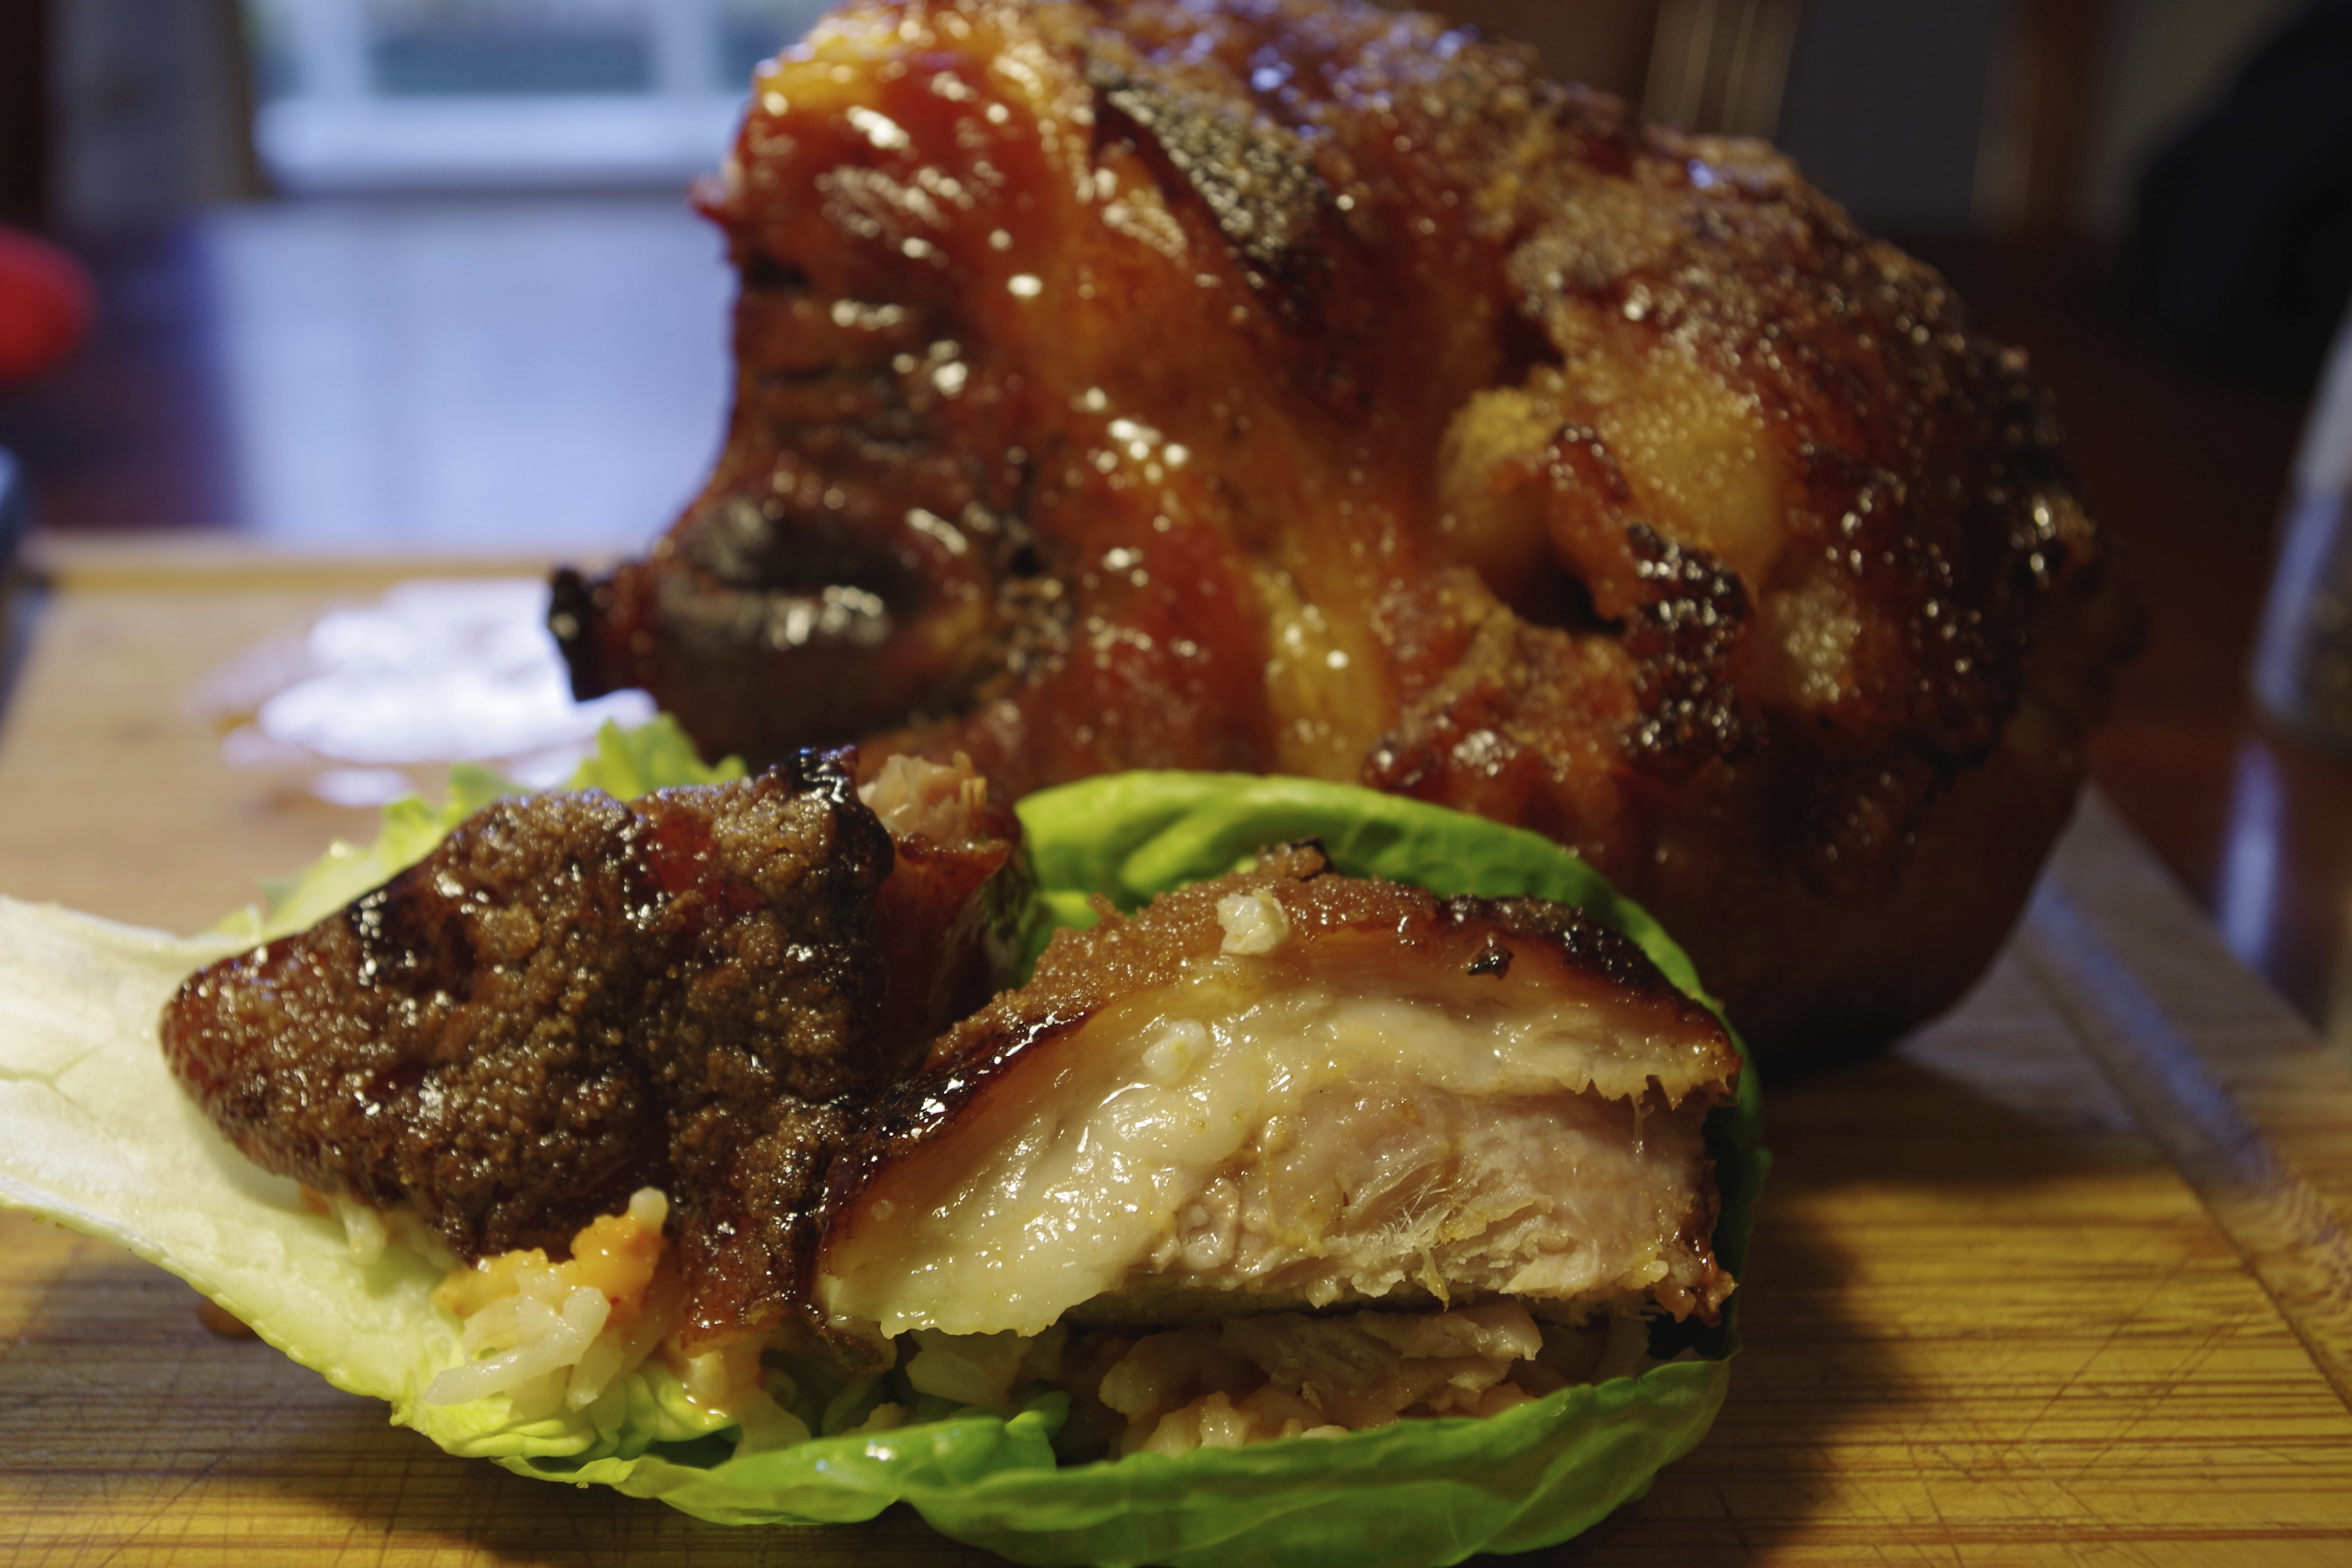
\includegraphics[width=\linewidth]{bossam.png}
\end{figure*}

\section{Bo Ssam}
\index{Pork!bo ssam}
\index{Mains!bo ssam}

This is a recipe for informal dinner parties: slow-roasted pork shoulder served with lettuce, rice and a raft of condiments. The recipe comes from  David Chang who runs the shrine to pork called  Momofuku in New York. This is a remarkably straightforward way to achieve high-level excellence with little more than ingredients and time. Simply cure the pork overnight beneath a shower of salt and some sugar, then roast it in a low oven until it collapses. Apply some brown sugar and a little more salt, then roast until it takes on the quality of glistening bark. Meanwhile, make the condiments; hot sauces and kimchi \& rice. Then tear meat off the bone and wrap it in lettuce, and keep at that until everything's gone.

\newpart{Pork butt (start the day before):}

\emph{1 whole bone-in pork butt or shoulder (3.5 to 4.5 kg)\sidenote{
You can either cut away the skin before cooking, or peel it off half way through. In the photo I peeled it off, but this leaves a much thicker layer of fat. Probably best to choose the method based on your cut.}
\\1 cup white sugar
\\1 cup plus 1 tbsp kosher salt\sidenote{
Kosher salt has a much larger grain than table salt, so half if not using kosher salt.}
\\7 tbsp brown sugar
}

\newpart{Ginger \& green onion sauce:}

\emph{2 1/2 cups whole green onions thinly sliced
\\1/2 cup minced ginger
\\1/4 cup neutral oil
\\2 tsp light soy sauce
\\1 tsp sherry vinegar
\\Salt to taste
}

\newpart{Ssam sauce:}

\emph{2 tbsp fermented bean-and-chili paste (ssamjang)
\\1 tbsp chilli paste (kochujang)
\\1/2 cup sherry vinegar
\\1/2 cup neutral oil
}

\newpart{Accompaniments:}

\emph{2 cups white rice
\\3 heads bendable lettuce
\\1 packet kimchi
\\1/2 cup neutral oil
}

\newpart{Pork:}
Place the pork in a large, shallow bowl. Mix the white sugar and 1 cup of the salt together in another bowl, then rub the mixture all over the meat. Cover it with plastic wrap and place in the refrigerator for at least 6 hours, or overnight.
When you're ready to cook, heat oven to 150\celsius. Remove pork from refrigerator and discard any juices. Place the pork in a roasting pan and set in the oven and cook for approximately 6 hours, or until it collapses, yielding easily to the tines of a fork. (After the first hour, baste hourly with pan juices.) At this point, you may remove the meat from the oven and allow it to rest for up to an hour.
When ready to serve, turn oven to 260\celsius. In a small bowl, stir together the remaining tablespoon of salt with the brown sugar. Rub this mixture all over the cooked pork. Place in oven for approximately 10 to 15 minutes, or until a dark caramel crust has developed on the meat. Serve hot, with the accompaniments.

\newpart{Accompaniments:}
For the green-onion and Ssam sauces - simply mix ingredients. 
Blend half the kimchi into a sauce, and serve the other half whole.
Prepare rice, wash lettuce and put kimchi and sauces into serving bowls.

%%%%%%%%%%%%%%%%%%%%%%%%%%%%%%%%%%%%%%%%%
\newpage

\begin{figure*}[h]
  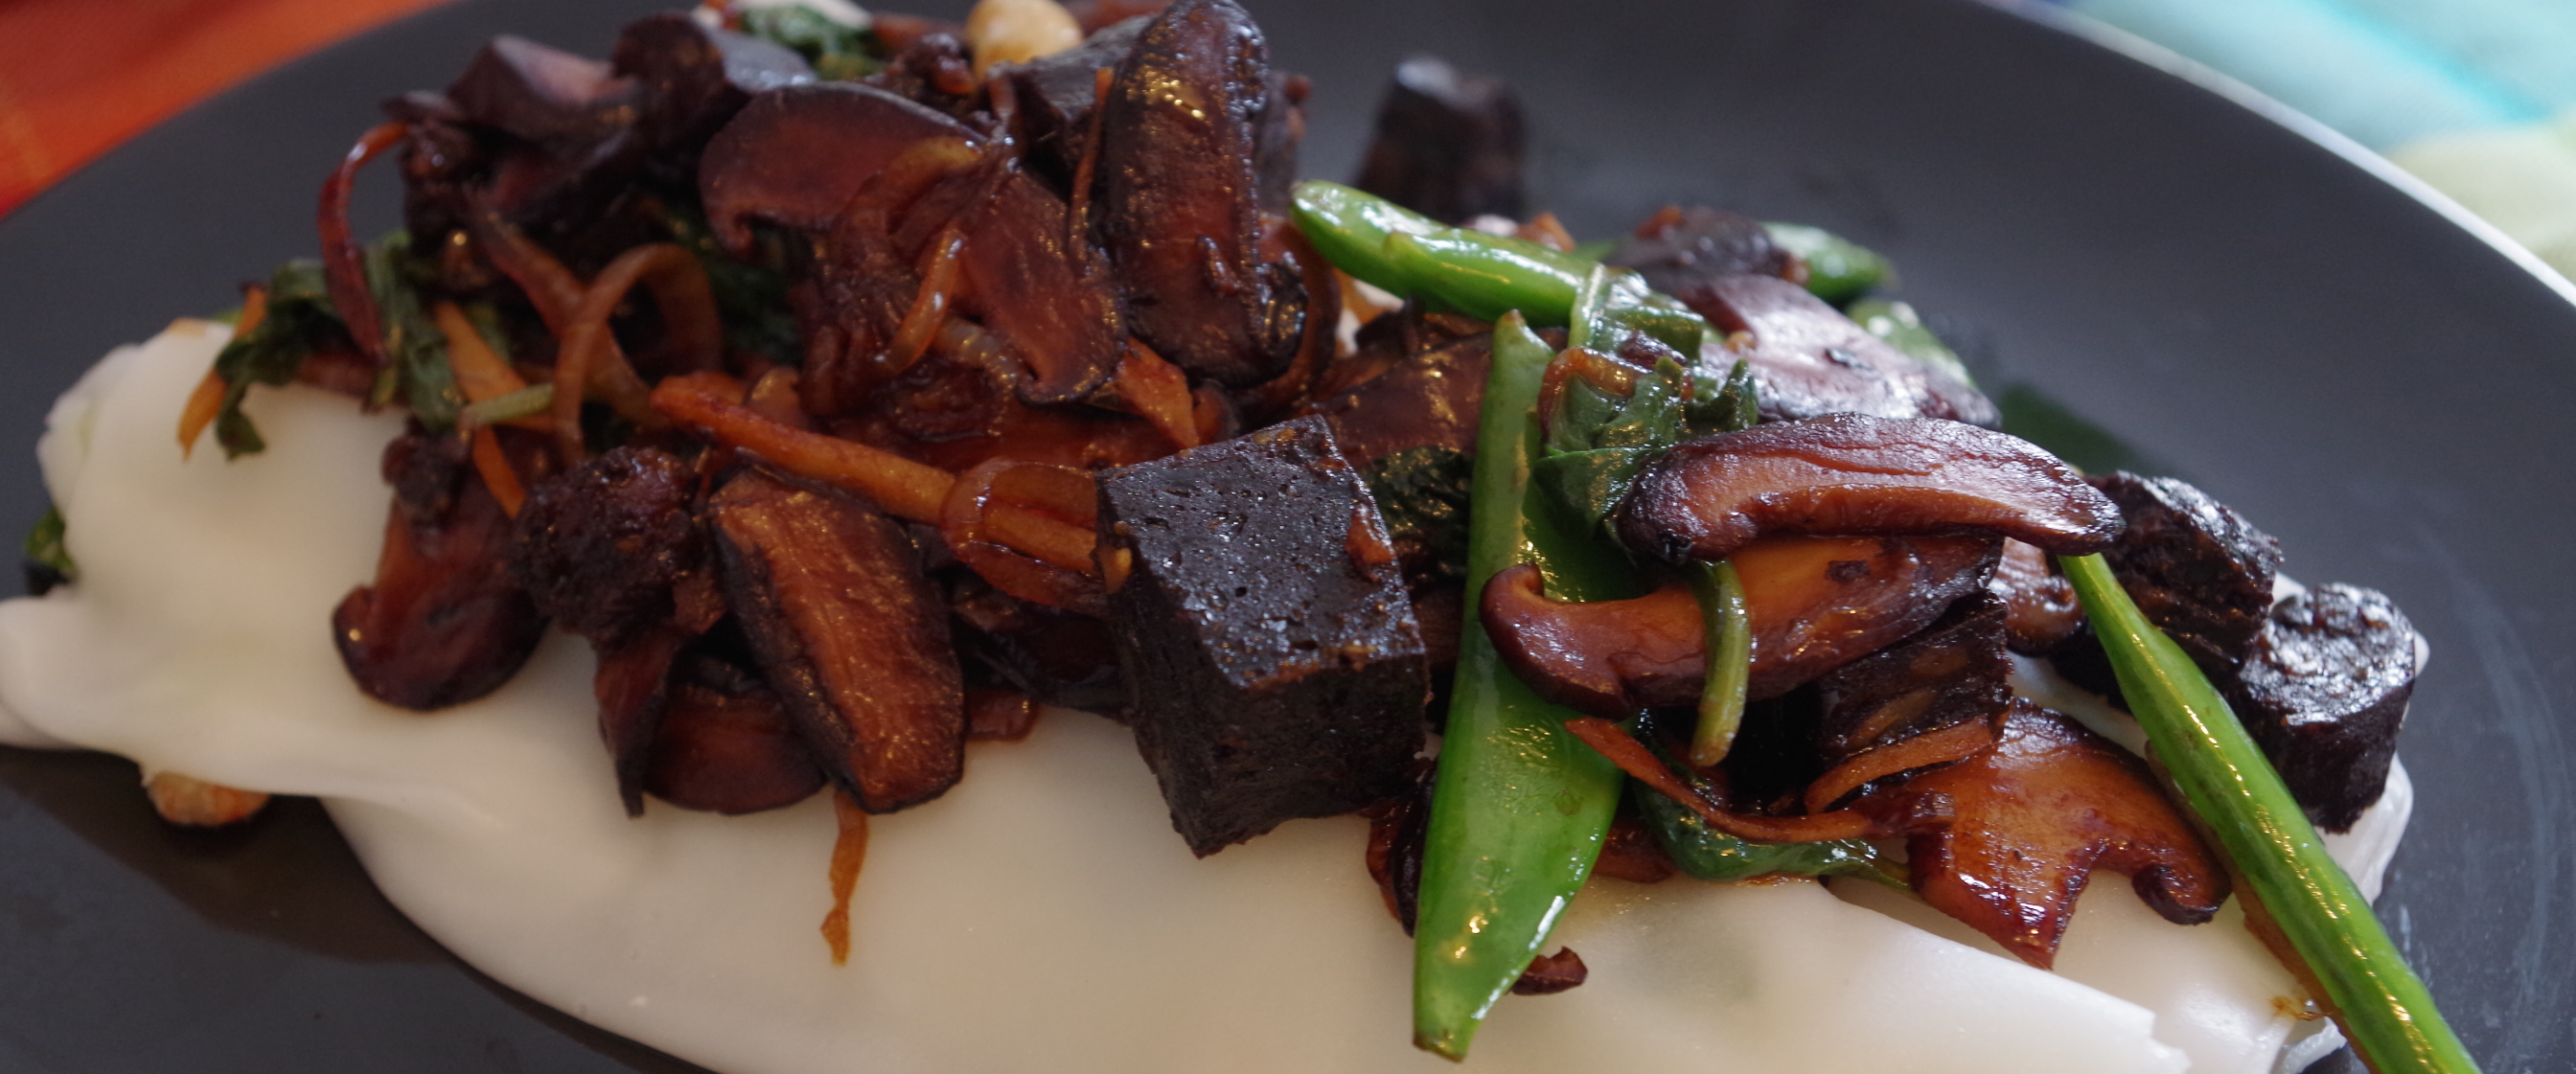
\includegraphics[width=\linewidth]{blackpuddingragout.JPG}
\end{figure*}

\section{Black pudding, pea, peanut, mushroom and spinach ragout}
\index{Mains!black pudding ragout}

This dish is a Scottish-Chinese hybrid, but it really works. The recipe comes from Peter Gordon at The Providores - a highly rated Kiwi restaurant in London.

\smallskip
\emph{200g black pudding
\\Peanut oil
\\Sesame oil
\\1 onion, peeled and thinly sliced
\\Big handful shitake mushrooms
\\Half thumb of ginger, julienned
\\50 ml mirin or 25ml rice wine vinegar
\\50 ml soy sauce
\\60 peanuts
\\100g spinach
\\100g peas
\\400g fresh rice noodles
}

\smallskip
Add the black pudding to a cold pan, and heat to medium high. Add a little oil if the black pudding isn't fatty. 
\\Once the black pudding is starting to go crispy, remove from the pan and add the oil, mushrooms and ginger. As it browns, add the soy sauce and wine vinegar.
\\Add the peanuts, spinach and peas with a heavy splash of water.\sidenote{
As soon as the spinach wilts it's ready. Add more water if needed so there is a little sauce.}
\\Heat the noodles in the microwave by pouring on some water and covering with cling film then serve.

%%%%%%%%%%%%%%%%%%%%%%%%%%%%%%%%%%%%%%%%%
\newpage

\begin{figure*}[h]
  \includegraphics[width=\linewidth]{chickenstuffed.png}
\end{figure*}

\section{Chicken roulade}
\index{Chicken!with pistachio}
\index{Chicken!poached}

This is based off a Gordon Ramsay recipe, but modified to take advantage of a sous vide machine.

\emph{4 chicken legs with thighs, or 8 thighs\sidenote{
Even chicken breasts can be used here.}
\\2 good quality raw sausages.
\\Big handful shelled pistachios
\\Saffron or paprika\sidenote{
Fake is fine, as the taste will be overpowered, and it's just wanted for the colour.}
\\3 3cm thick slices of butter
}

\begin{marginfigure}%
  \includegraphics[width=\linewidth]{stuffingchicken.jpg}
\end{marginfigure}

Debone and skin the chicken, you want it to be around 1-2cm thick. 
Lay out some gladwrap, then place the three pats of butter on it, and season it with salt, pepper and pinches of either paprika or saffron. Then lay the chicken on top.  
Then mix the sausage with the pistachios and lay it like it is in the picture in the sidebar. Then, roll up tightly with lots of gladwrap, and, it you don't trust your wrapping, also place in a freezer bag.
When you're ready to cook, place the chicken roll into the sous vide machine at 60\celsius   for 2-3 hours. Anytime after two hours, slice to serve.

\newpart{Optional accompaniments:}
I roasted the bones to make a gravy, and also placed the skins between two baking sheets (between layers of wax paper), in an oven at 190\celsius  for 50 minutes to make chicken skin crackling.


%%%%%%%%%%%%%%%%%%%%%%%%%%%%%%%%%%%%%%%%%%%%%%%%%%%%
\newpage

\begin{figure*}[h]
  \includegraphics[width=\linewidth]{jerkchicken.JPG}
\end{figure*}

\section{Jerk chicken}
\index{Mains!jerk chicken}
\index{Chicken!jerk}

\smallskip
\emph{1 tbsp allspice
\\1 tbsp black pepper
\\1/2 tbsp muscovado sugar
\\2 tbsp honey
\\A few sprigs fresh coriander
\\2 chillies
\\1 clove garlic
\\3 cm piece fresh ginger, peeled
\\2 spring onions, trimmed and finely sliced
\\2 big lugs olive oil
\\8 chicken thighs}

\smallskip
Heat the oven to 100\celsius.
\\Blend all the ingredients except the chicken to a paste.
\\Rub into the chicken, place in a covered oven dish for around 3 hours.
\\After 3 hours, either immediately grill to crisp the skin, or chill in the fridge for grilling later on a BBQ.

%%%%%%%%%%%%%%%%%%%%%%%%%%%%%%%%%%%%%%%%%%%%%%%%%%%%
\newpage

\begin{figure*}[h]
  \includegraphics[width=\linewidth]{greekchicken.JPG}
\end{figure*}

\section{Greek chicken}
\index{Mains!Greek chicken}
\index{Chicken!Greek}

A relatively easy, fresh and interesting dish.

\smallskip
\emph{600g boneless, skinless, chicken thighs
\\5 tbsp olive oil
\\1 tbsp dried oregano
\\2 cloves crushed garlic
\\1 tsp ground cumin
\\1 red capsicum, thinly sliced
\\1 red onion, thinly sliced
\\400gm tin of chickpeas, rinsed
\\12 cherry tomatoes
\\1/2 cup raisins
\\Handful of olives
\\100g feta, crumbled
\\Mint to garnish
}

\smallskip
Mix the honey and soy and pour it into a cold pan with the chicken.
\\Turn on the element to medium and cook till the sauce is reduced and chicken cooked (around 30 mins).

\newpart{1 to 12 hours before:} 
\\Chop the chicken into cubes then marinade for at least a few hours hours in the olive oil, oregano, garlic and cumin. 
\\\newpart{20 mins before:} 
\\Fry chicken in the wok in batches until fully cooked. Drain and keep warm.
\\Fry the capsicum and onion until just tender.
\\Add the chickpeas, tomatoes and raisins and cook for 3 or 4 minutes. Season if necessary.
\\Add the chicken and any of the meat juices and the olives and cook for 1 to 2 minutes. Season if necessary.
\\Transfer to a dish and add herbs and feta
\\Serve with a good bread or couscous.

%%%%%%%%%%%%%%%%%%%%%%%%%%%%%%%%%%%%%%%%%%%%%%%%%%%%

\begin{figure*}[h]
  \includegraphics[width=\linewidth]{stickychicken.png}
\end{figure*}

\section{Honey soy chicken}
\index{Mains!honey soy chicken}
\index{Chicken!honey soy}

The easiest recipe ever! Serves 2.

\smallskip
\emph{2 tbsp honey
\\2 tbsp soy sauce
\\4 skinned and boned chicken thighs\sidenote{Chicken legs can also be used, like in the photo, just remember to brown them quickly first or remove the skin.}}

\smallskip
Mix the honey and soy and pour it into a cold pan with the chicken.
\\Turn on the element to medium and cook till the sauce is reduced and chicken cooked (around 30 mins).

%%%%%%%%%%%%%%%%%%%%%%%%%%%%%%%%%%%%%%%%%%%%%%%%%%%%
\newpage

\begin{figure*}[h]
  \includegraphics[width=\linewidth]{friedchicken.jpg}
\end{figure*}

\section{Fried chicken sandwich}
\index{Mains!fried chicken}
\index{Chicken!fried}

\smallskip
\emph{8 soft/pretzel or steamed rolls
\\1 small yellow onion, coarsely grated
\\2 cloves garlic, minced
\\1/2 teaspoon salt, plus more for coating
\\1/4 teaspoon black pepper, plus more for coating
\\8 boneless, skinless chicken thighs
\\3 tablespoons Korean chili paste (gojuchang)
\\Oil for deep frying
\\1/2 cup all-purpose flour 
\\2/3 cup cornstarch}

\smallskip
In a medium-size bowl, combine grated onion, garlic, salt and pepper and chili paste. Add chicken and toss to coat well. Cover and set aside to marinate for about 1 hour.
\\Pour oil into a large heavy pot to a depth of 1-2cm. Heat to 350\celsius. Combine flour and cornstarch in a shallow bowl and season with salt and pepper.
\\Working in batches to avoid crowding, lift chicken from marinade, dredge lightly in seasoned flour and cornstarch, gently drop into oil and fry for 5 to 7 minutes, turning occasionally, until golden brown and crisp. 
\\Drain on paper towels. Repeat with remaining chicken, checking oil temperature between batches.

%%%%%%%%%%%%%%%%%%%%%%%%%%%%%%%%%%%%%%%%%%%%%%%%%%%%
\newpage

\begin{figure*}[h]
  \includegraphics[width=\linewidth]{chickendoner.JPG}
\end{figure*}

\section{Chicken doner}
\index{Mains!chicken doner}
\index{Chicken!doner}

A healthier take on the doner. Goes well with shredded lettuce, tomatoes, feta, pita bread and a tahini yoghurt sauce. Serves 4-5.

\smallskip
\emph{2 lemons, juiced
\\1/2 cup olive oil
\\6 cloves garlic, peeled, smashed and minced
\\1 tsp kosher salt
\\2 tsp each of ground cumin, paprika, tumeric, pepper
\\Red-pepper flakes, to taste
\\900g boneless, skinless chicken thighs
\\2 large red onions, peeled and quartered
\\2 tbsp chopped fresh parsley}

\smallskip
\newpart{1 to 12 hours before:} 
\\Combine the lemon juice, 1/2 cup olive oil, garlic, salt, pepper, cumin, paprika, turmeric, cinnamon and red-pepper flakes in a large bowl, with the chicken. Marinade for 1 to 12 hours.
\\\newpart{When ready to cook:} 
\\Preheat oven to 220\celsius. Add the quartered onions to the chicken and marinade, and toss once to combine. Place everything in a rimmed oven tray and roast until it is browned (about 30 to 40 minutes). Remove from the oven, allow to rest 2 minutes, then slice into bits. Scatter the parsley over the top.

%%%%%%%%%%%%%%%%%%%%%%%%%%%%%%%%%%%%%%%%%%%%%%%%%%%%
\newpage

\begin{figure*}[h]
  \includegraphics[width=\linewidth]{lambwithmint.png}
\end{figure*}

\section{Lamb with mustard and mint}
\index{Lamb!with mustard and mint}
\index{Mains!lamb with mustard and mint}

A simple dish of lamb, slow roasted. It will seem like too much water, but trust the recipe, as it will all evaporate. Goes well with polenta. Serves 6.

\smallskip
\emph{6 Lamb neck fillets
\\Large handfull mint
\\80ml olive oil
\\3 tbsp wholegrain mustard
\\3 tbsp soy sauce
\\3 tbsp Worcestershire sauce
\\1.5L water}

\smallskip
Preheat oven to 180\celsius. Pick the mint leaves from the stalks. 
\\Season the lamb with salt and pepper, then brown in the olive oil.
\\Place in roasting dish, cover with mustard, soy sauce, Worcestershire sauce, and 80\% of the mint then pour in water. 
\\Seal with foil and roast for 3 hours, turning roughly every 45 mins.
\\Finely chop the remaining mint as a garnish.

%%%%%%%%%%%%%%%%%%%%%%%%%%%%%%%%%%%%%%%%%%%%%%%%%%%
\newpage

\begin{figure*}[h]
  \includegraphics[width=\linewidth]{gnocchi.png}
\end{figure*}

\section{Gnocchi with celery leaves and w{\"u}rst}
\index{Mains!gnocchi}
\index{W{\"u}rst!with gnocchi}

A great way to use up celery leaves.

\smallskip
\emph{One packet of gnocchi
\\Several large handfuls of finely sliced celery leaves
\\One sausage\sidenote{Either sliced, or squeezed out of the casing as meat balls}
\\One tablespoon of mustard
\\100ml of creme or soft cheese}

\smallskip
Brown the w{\"u}rst in a pan with a little oil.
\\Meanwhile, throw the gnocchi into a pan of boiling water, then drain when the gnocchi raises the top of the water. This should just take a few minutes.
\\As the sausage browns, throw in the celery leaves.
\\When the celery has softened add in the cooked gnocchi and cream.
\\Stir for a few minutes, making sure to scrub the tasty bits of the pan.
\\Just before eating, stir in the mustard.


%%%%%%%%%%%%%%%%%%%%%%%%%%%%%%%%%%%%%%%%%%%%%%%%%%%
\newpage

\begin{figure*}[h]
  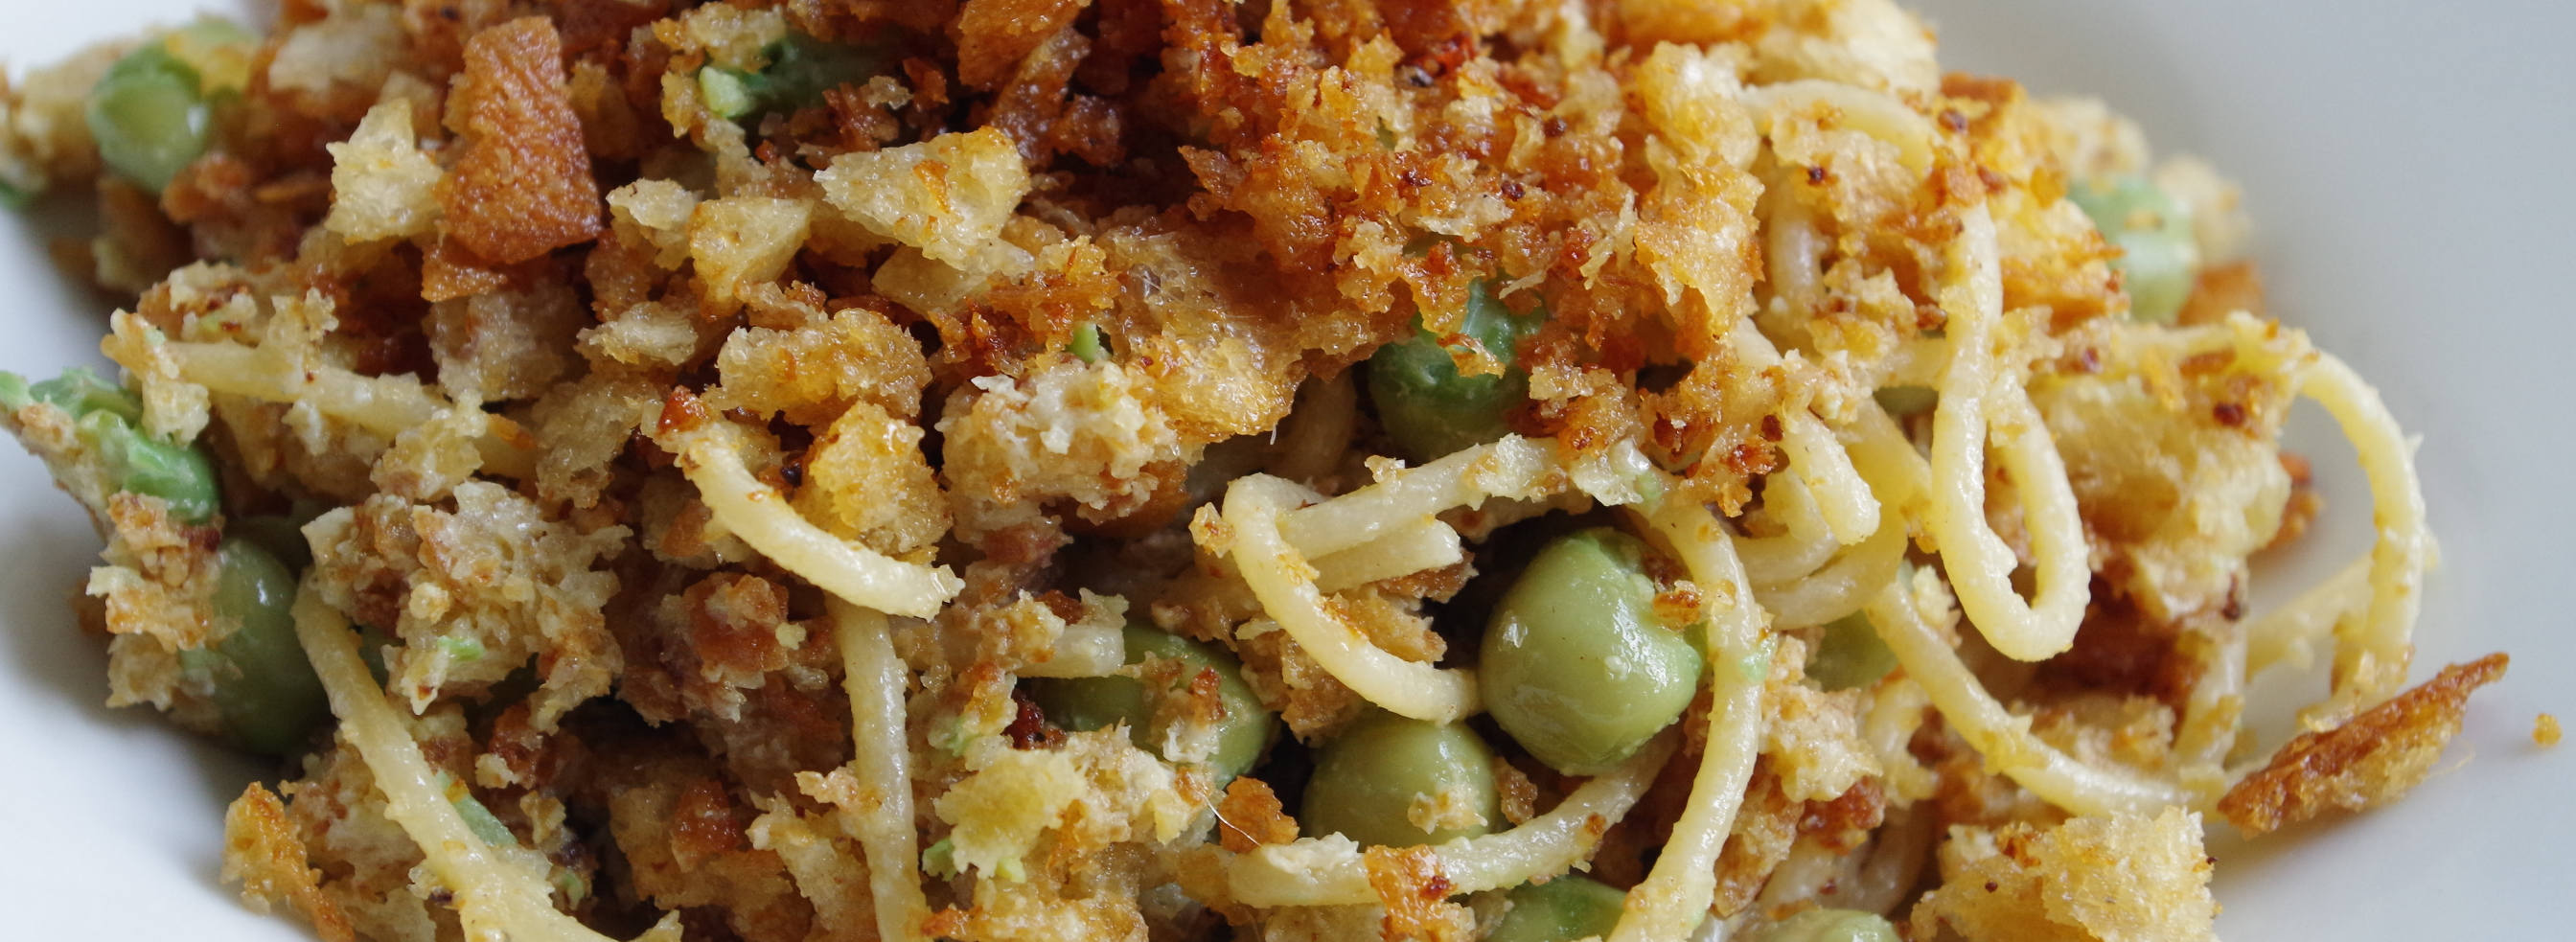
\includegraphics[width=\linewidth]{breadcrumbpasta.png}
\end{figure*}

\section{Anchovy and breadcrumb pasta }
\index{Mains!pasta}
\index{Pasta!Anchovy and breadcrumb}

A great store cupboard recipe - if you have bread, you probably have all the ingredients needed. With good quality olive oil it's an amazing dinner.

\smallskip
\emph{Spaghetti or linguine for three
\\1/3 cup extra-virgin olive oil, more as needed
\\12 anchovies, chopped\sidenote{
Can also add a tbsp of fish sauce to boost the umami}
\\6 garlic cloves, minced
\\1/4 teaspoon red pepper flakes
\\1 cup good dried bread crumbs
\\2 egg yolks
\\1 teaspoon hot sauce, such as Tabasco, or to taste
\\1/2 cup roughly chopped parsley
\\Lemon wedges, for serving}

\smallskip
Over medium-high heat, warm oil. Add anchovies, garlic and red pepper flakes; cook until fragrant, 1 minute. Stir in bread crumbs and cook until golden, 2 to 3 minutes. Season liberally.
\\Cook the pasta; drain well, reserving some of the pasta water (about 1/2 cup is plenty).\sidenote{You can frozen peas just before the pasta is cooked if you want some veges.} 
\\Stir together egg yolks, hot sauce and 2 tablespoons pasta water. Add hot pasta and toss well, adding more pasta water if the mixture looks dry or unevenly yellow. You want the yolk to evenly coat the pasta but you don't want it to be soupy. Add bread crumb mixture and parsley and toss well. Season and serve with lemon wedges.


%%%%%%%%%%%%%%%%%%%%%%%%%%%%%%%%%%%%%%%%%
\newpage

\begin{figure*}[h]
  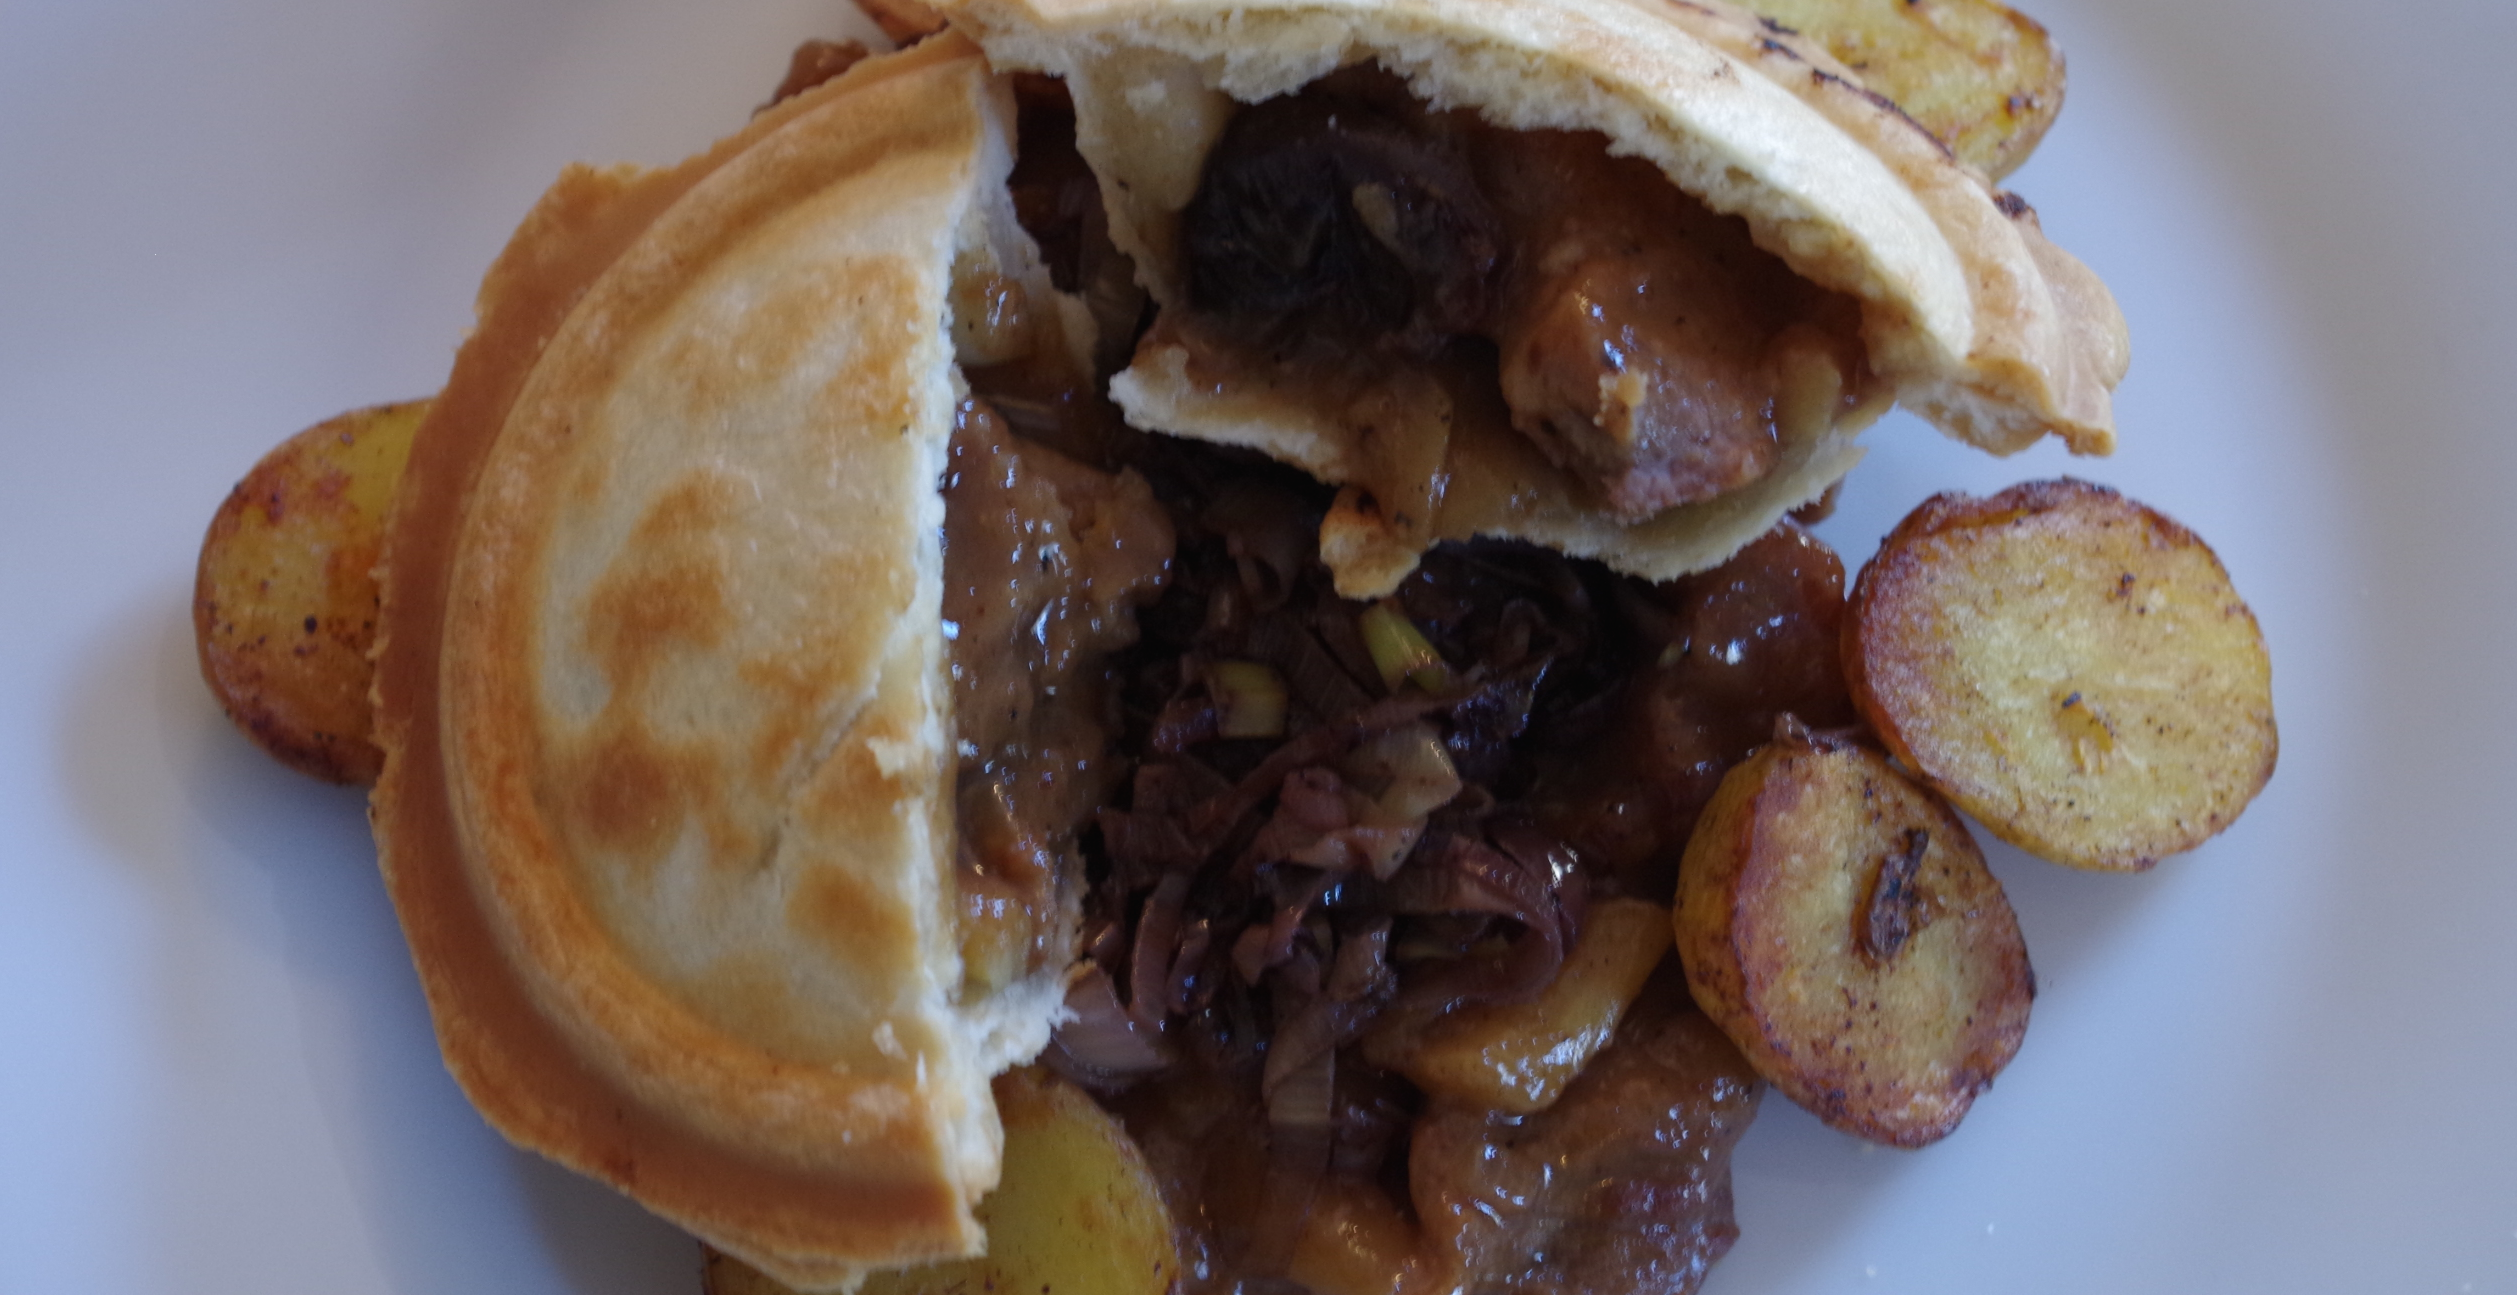
\includegraphics[width=\linewidth]{porkpie.png}
\end{figure*}

\section{Pork and Prune Pie}
\index{Mains!pork pie}
\index{Pie!pork \& prune}
\index{Pork!\& prune}
\index{Stew!pork and prune}

This is a super easy, and tasty stew that doesn't have to served in a pie. The fruit makes it quite rich, so in lieu of pastry it needs something like mashed potatoes as a side. Serves at least four.

\smallskip
\emph{400g diced pork
\\2 tbsp flour
\\2 tbsp oil
\\1 onion, diced finely
\\4 apples, peeled and chopped
\\2 cloves garlic
\\2 cups apple juice or cider
\\150g pitted prunes
\\Shortcrust pastry packet
\\4 tbsp milk}

\smallskip
Toss pork in flour and fry until lightly brown, then put aside.
\\Fry onion, garlic and apple for 3 minutes.
\\Add apple juice or cider to deglaze, then add the prunes.
\\Cook on low for about an hour, then let it cool with the pan off the heat.
\\When cold (or at least cool-ish), make pie and glaze pastry with milk.

%%%%%%%%%%%%%%%%%%%%%%%%%%%%%%%%%%%%%%%%%
\newpage

\begin{figure*}[h]
  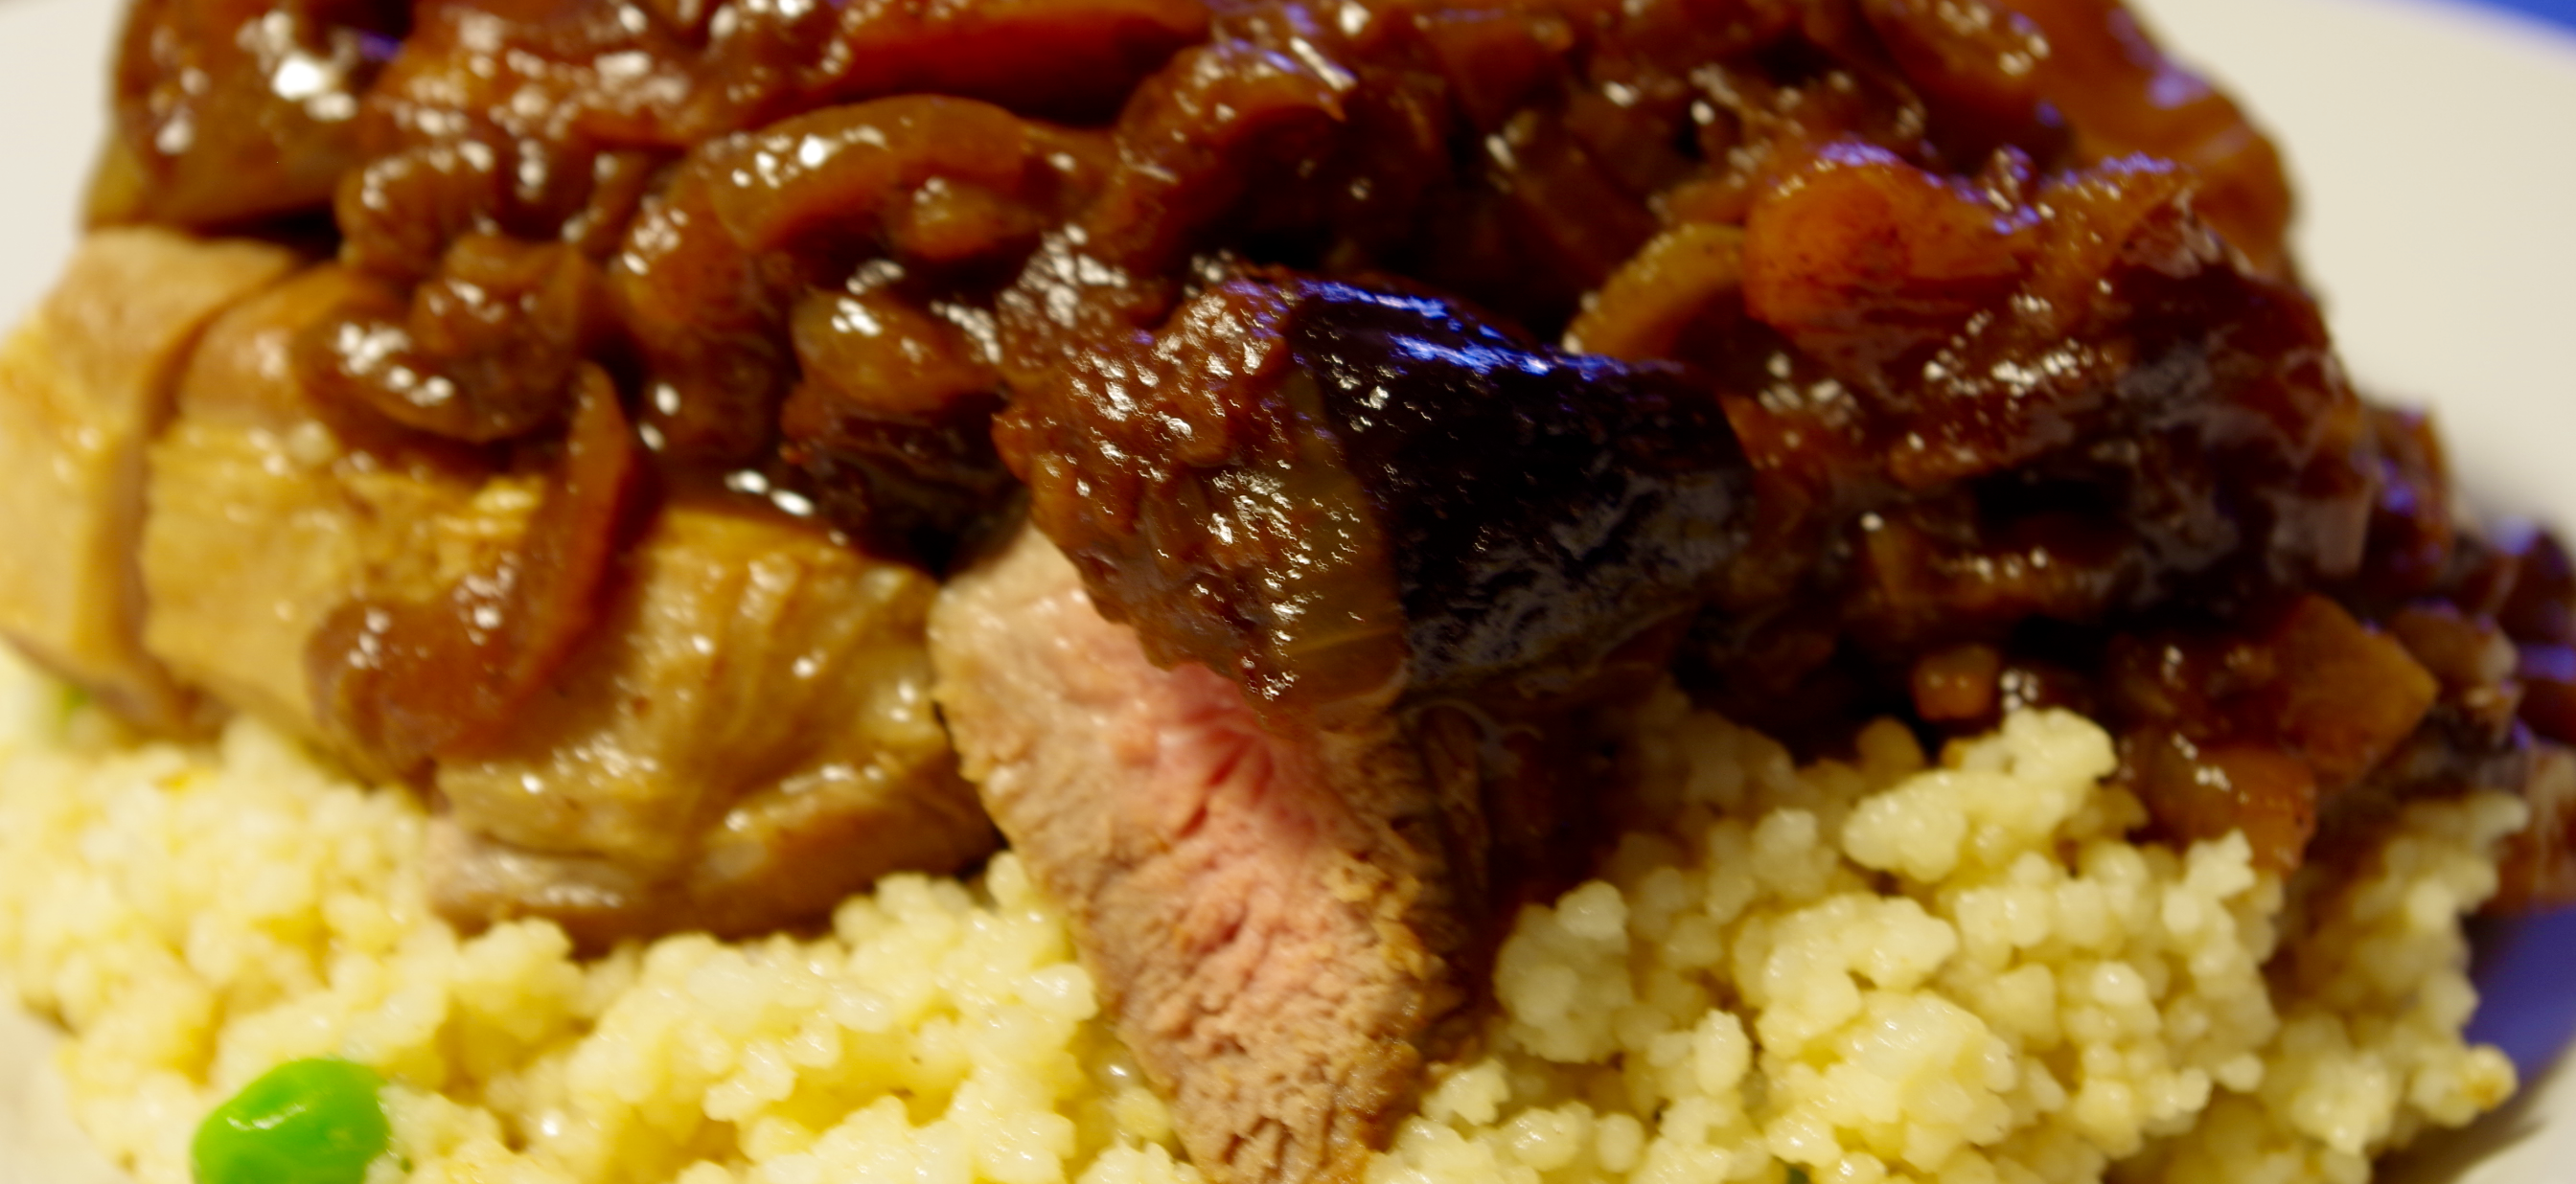
\includegraphics[width=\linewidth]{lambtagine.png}
\end{figure*}

\section{Moroccan lamb}
\index{Mains!Moroccan lamb}
\index{Lamb!Moroccan stew}
\index{Stew!Moroccan}

\emph{1 kg lamb in 4 cm cubes
\\2 onions
\\15g butter
\\2 tbsp oil
\\1 tsp black pepper
\\1 cinnamon stick
\\1 1/2 tbsp honey
\\2 tsp ground ginger
\\2 tsp ground cumin
\\1 1/2 tbsp ground cinnamon
\\200g dried apricots
\\200g prunes
\\2 long strips lemon rind}

\smallskip
Remove all fat from lamb then sear in butter, and remove.
\\Add spices and onion and fry till soft.
\\Add lamb back in, top with water till 1cm up pan, cover and simmer for an hour.
\\Remove lid, add lemon rind, honey, cinnamon, and fruit and simmer for 30mins with the lid off.\sidenote{
Becareful of it suddenly thickening thanks to the prunes, as it will stick.}

%%%%%%%%%%%%%%%%%%%%%%%%%%%%%%%%%%%%%%%%%%%%%%%%%%%%
\newpage


\begin{figure*}[h]
  \includegraphics[width=\linewidth]{paella.png}
\end{figure*}

\section{Paella}
\index{Mains!paella}
\index{Rice!paella}
\index{Seafood!paella}

An easy dinner party dish as you can make it 90\% before hand, then just add the shellfish and reheat to serve.

\begin{marginfigure}%
  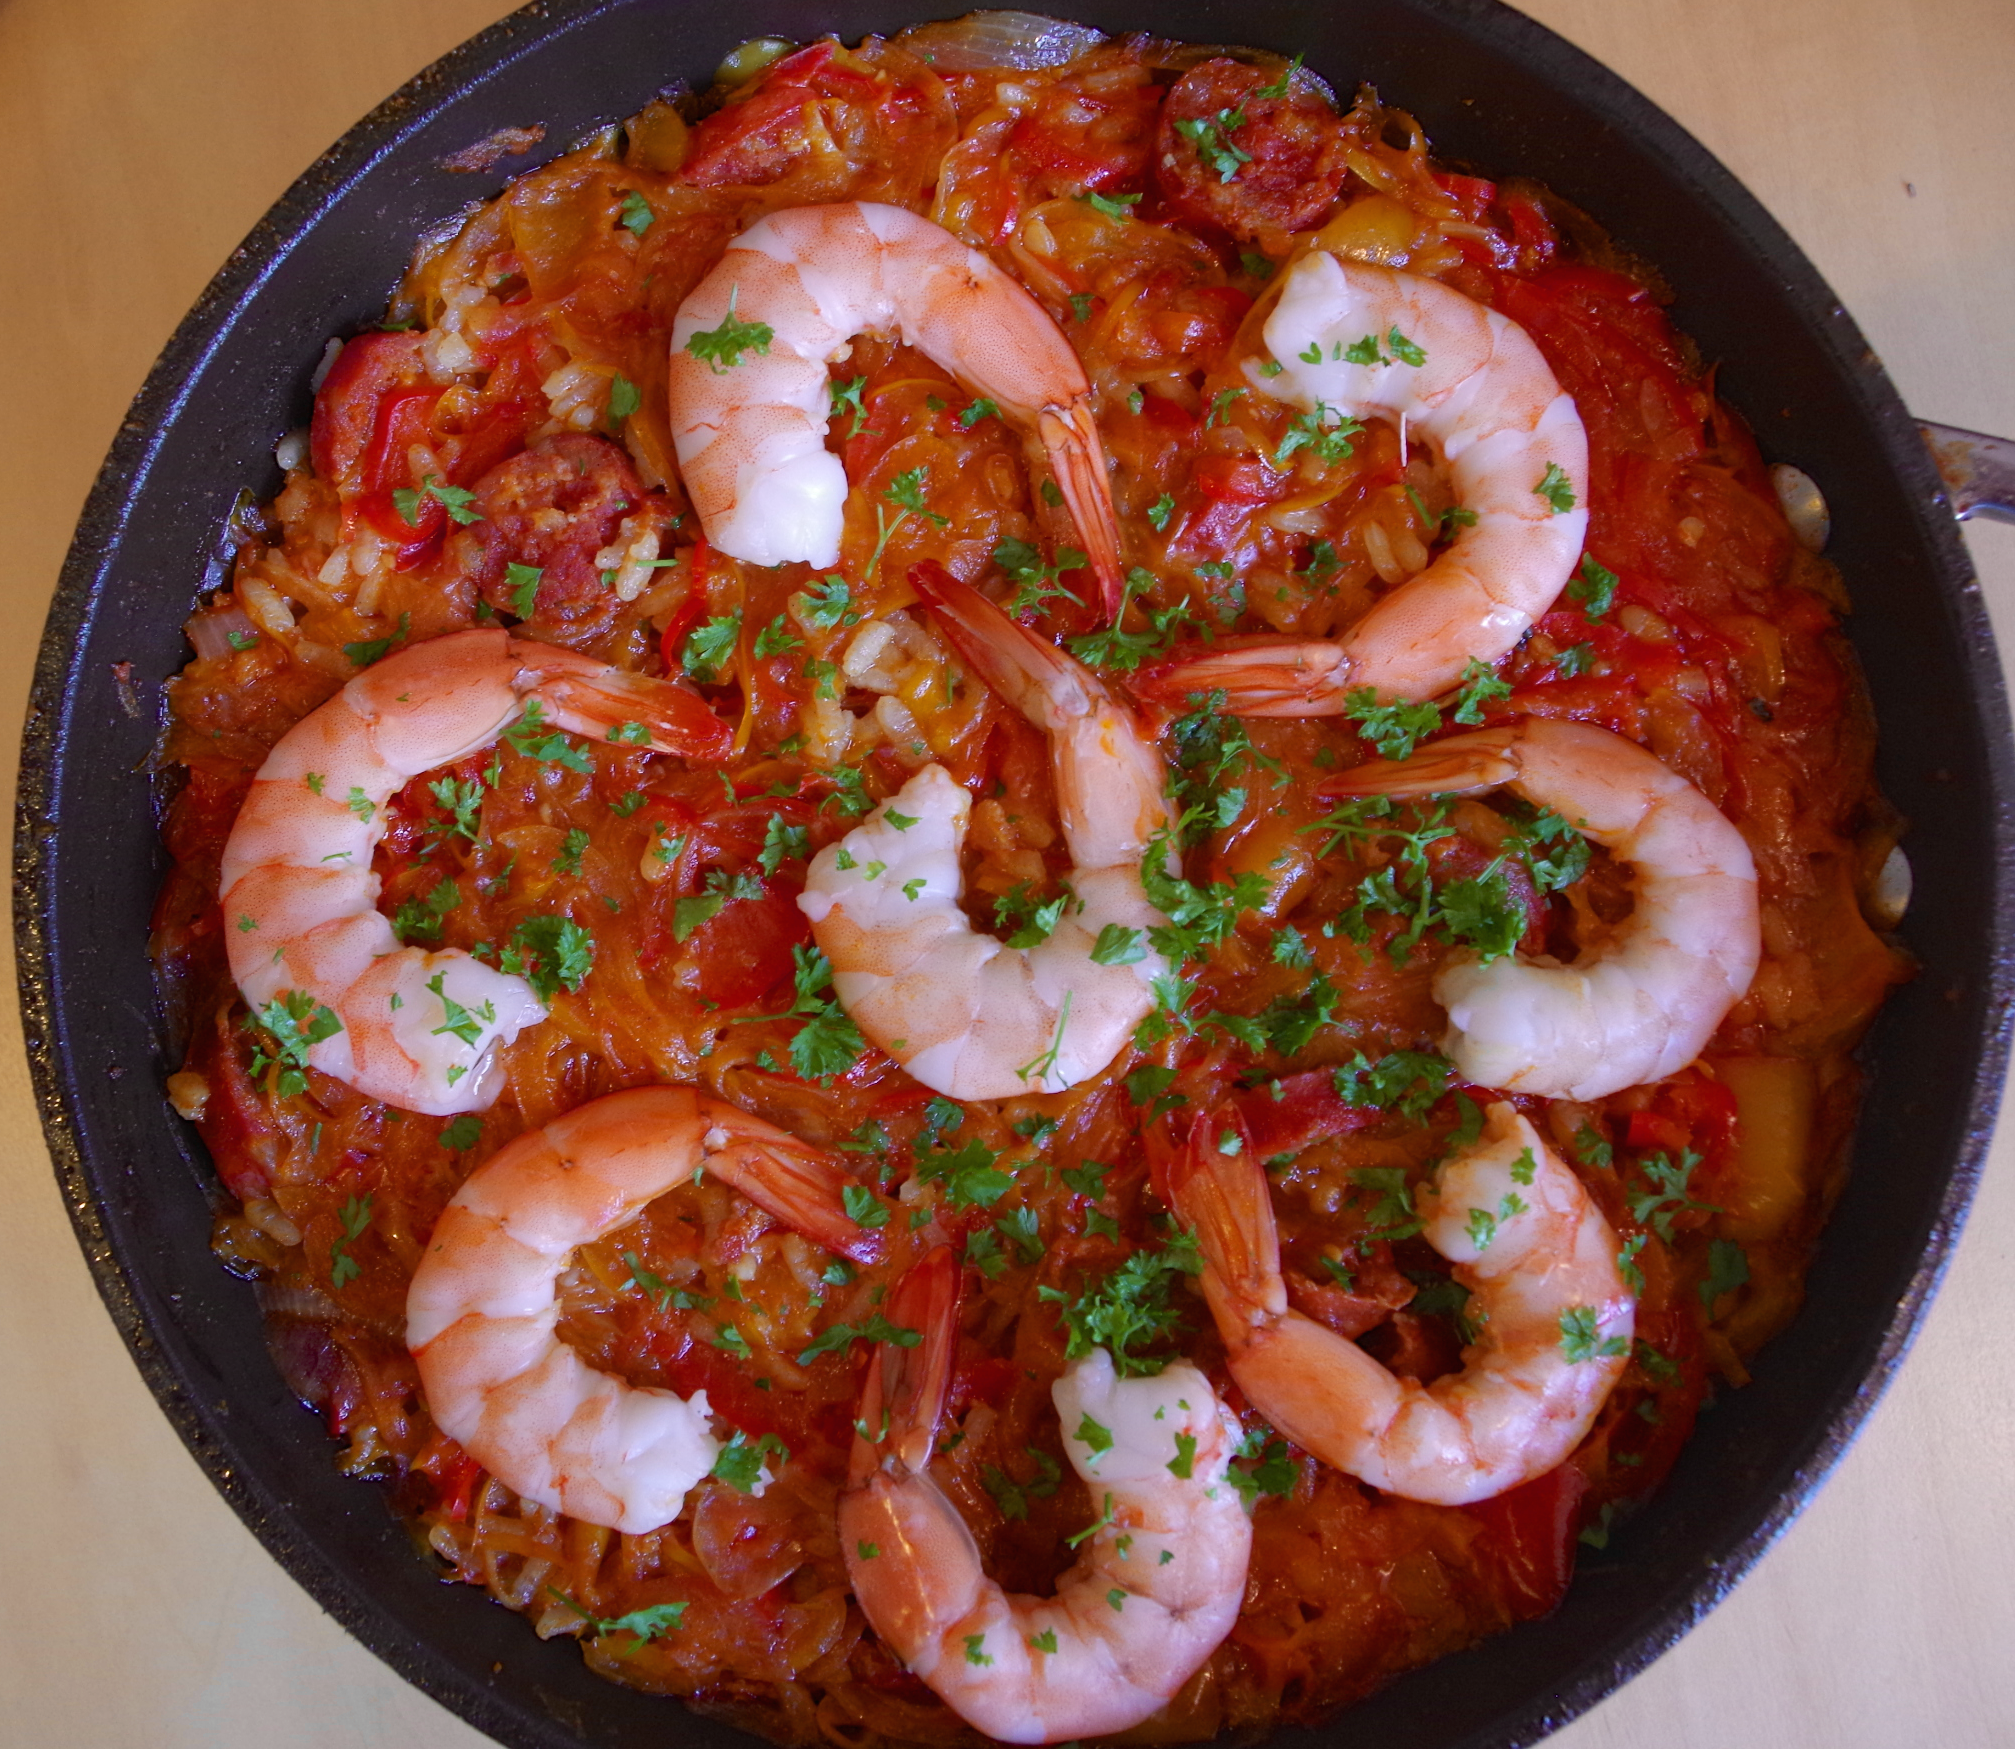
\includegraphics[width=\linewidth]{paellahigh.png}
\end{marginfigure}

\smallskip
\emph{250g tomatoes, with x in top\sidenote{Or half a tin of tomatoes}
\\100ml olive oil
\\6 chicken thighs\sidenote{You can easily omit either the chicken or prawns}
\\220g chorizo, sliced
\\1 onion, finely chopped
\\2 peppers (any colour), finely chopped
\\2 cloves garlic
\\1 1/2 tsp sweet paprika
\\1/2 tsp cayanne pepper
\\350g paella rice
\\1.2L stock
\\75g fresh peas
\\12 tiger prawns
\\3 tbsp chopped flat-leaf parsely leaves
\\Finely chopped zest and juice of one lemon
}

\smallskip
Boil the tomatoes for 10 seconds then skin and deseed.
\\Heat the oil in a large frying pan to medium and fry the chicken skin side down till dark brown with the chorizo.
\\Remove the chicken and add chorizo.\sidenote{I like to blend 1/3 of the chorizo so it melts into the paella, but that's completely optional and probably heresy.}
\\Soon after, add the peppers and garlic and fry for 3 minutes.
\\Add the spices and rice.
\\After a few minutes, once the rice starts to go clear, add the stock and tomatoes and bring to the boil.\sidenote{If you deheaded the shrimp, I like to add it to the stock while it's heating (discard before adding to the paella).}
\\Turn the heat to low and simmer for 15 minutes with the lid off.
\\Then add back the chicken, with the prawns and peas, and cook for 15 more minutes.\sidenote{If the prawns are large, turn them once by hand to make sure they cook through.}
\\Squeeze over a lemon and sprinkle with zest and juice.


%%%%%%%%%%%%%%%%%%%%%%%%%%%%%%%%%%%%%%%%%%%%%%%%%%%%
\newpage

\section{Phat thai}
\index{Mains!phat thai}
\index{Noodles!phat thai}

Phat thai and I have a weird relationship. Like how hollandaise becomes less appealing when you make it yourself (and see all the butter) - I can't seem to make good phat thai without a lot of oil. It's still a great, and easy dish to make - it just needs a lot of ingredients.

\smallskip
\emph{120g 2-3mm wide flat rice sticks
\\60ml fish sauce
\\60ml tamarind water
\\60g palm sugar
\\Pinch of chilli powder, to taste
\\80ml groundnut or vegetable oil
\\2 cloves of garlic, finely chopped
\\100g extra-firm tofu, chopped into small cubes
\\8 large prawns
\\2 large eggs, ready cracked
\\1 tbsp small dried shrimp
\\100g beansprouts
\\4 stalks Chinese chives, chopped
\\50g roasted peanuts, roughly chopped
\\Lime wedges, chilli flakes, fish sauce and sugar, to garnish}

\smallskip
Soak the rice sticks in cold water for about half an hour until pliable but al dente. Drain.
\\Meanwhile, make the sauce by combining the fish sauce, tamarind and palm sugar in a small pan. Heat gently to dissolve the sugar and taste. Add more of any of the ingredients as you wish. Season with chilli to taste. Set aside.
\\Lay out all the ingredients within easy reach of the hob in the order they'll be used. Put a wok on a high heat and add half the oil. Add the garlic, stir fry for a few seconds, then add the noodles and a splash of water. Stir fry until they're drying out, then add the sauce. Fry until they are almost soft enough to eat (they should be slightly chewy).
\\Push the noodles to the side of the wok and add the rest of the oil. Fry the tofu and prawns until the tofu is beginning to colour, then push to the side and add the eggs. Pierce the yolks and, when starting to set on the bottom, scramble.
\\Stir through the noodles, and add the radish, dried shrimp, beansprouts, chives and peanuts. Stir fry until well combined, then serve with the garnishes for people to add as they wish.

%%%%%%%%%%%%%%%%%%%%%%%%%%%%%%%%%%%%%%%%%
\newpage


\begin{figure*}[h]
  \includegraphics[width=\linewidth]{fleurs.JPG}%
\end{figure*}

\section{Fleur's fish rarebit}
\index{Fish!rarebit}

\emph{2 fillets of boned, skinned, white fish
\\50g flour
\\50g butter
\\200ml of beer
\\1 tbsp mustard
\\1 tbsp Worcestershire sauce
\\100g of strong cheddar cheese\sidenote{
You can also use any strong cheese.}
\\1 egg yolk
\\5 cloves garlic
\\Packet spinach leaves
\\2 eggs
\\Vinegrette
}

\smallskip
\newpart{The day before:} 
\\On a low heat, melt the butter and stir in the flour to make a roux. Heat the ale, but do not let it boil, and add it to the mix, stirring gently and constantly over a low heat.
\\Melt the cheese in a bowl placed over a pan of boiling water. When melted, pour into the mixture. Stir once to amalgamate, then remove from the heat.
\\Add the Worcestershire sauce, mustard, egg yolk, salt and pepper, then transfer to a food processor and blitz until the rarebit mixture has formed an emulsion. Transfer to a bowl, allow to cool, then refrigerate.
\\\newpart{On the day:} 
Heat the oven to 200\celsius. Take your Welsh rarebit mixture out of the fridge and spread on the fish, then bake for 20 mins.
\\Boil the eggs, and serve with the fish as on top of the spinach.\sidenote{Soft boiled if possible - I got distracted cooking the ones in the photo.}

%%%%%%%%%%%%%%%%%%%%%%%%%%%%%%%%%%%%%%%%%
\newpage

\begin{figure*}[h]
  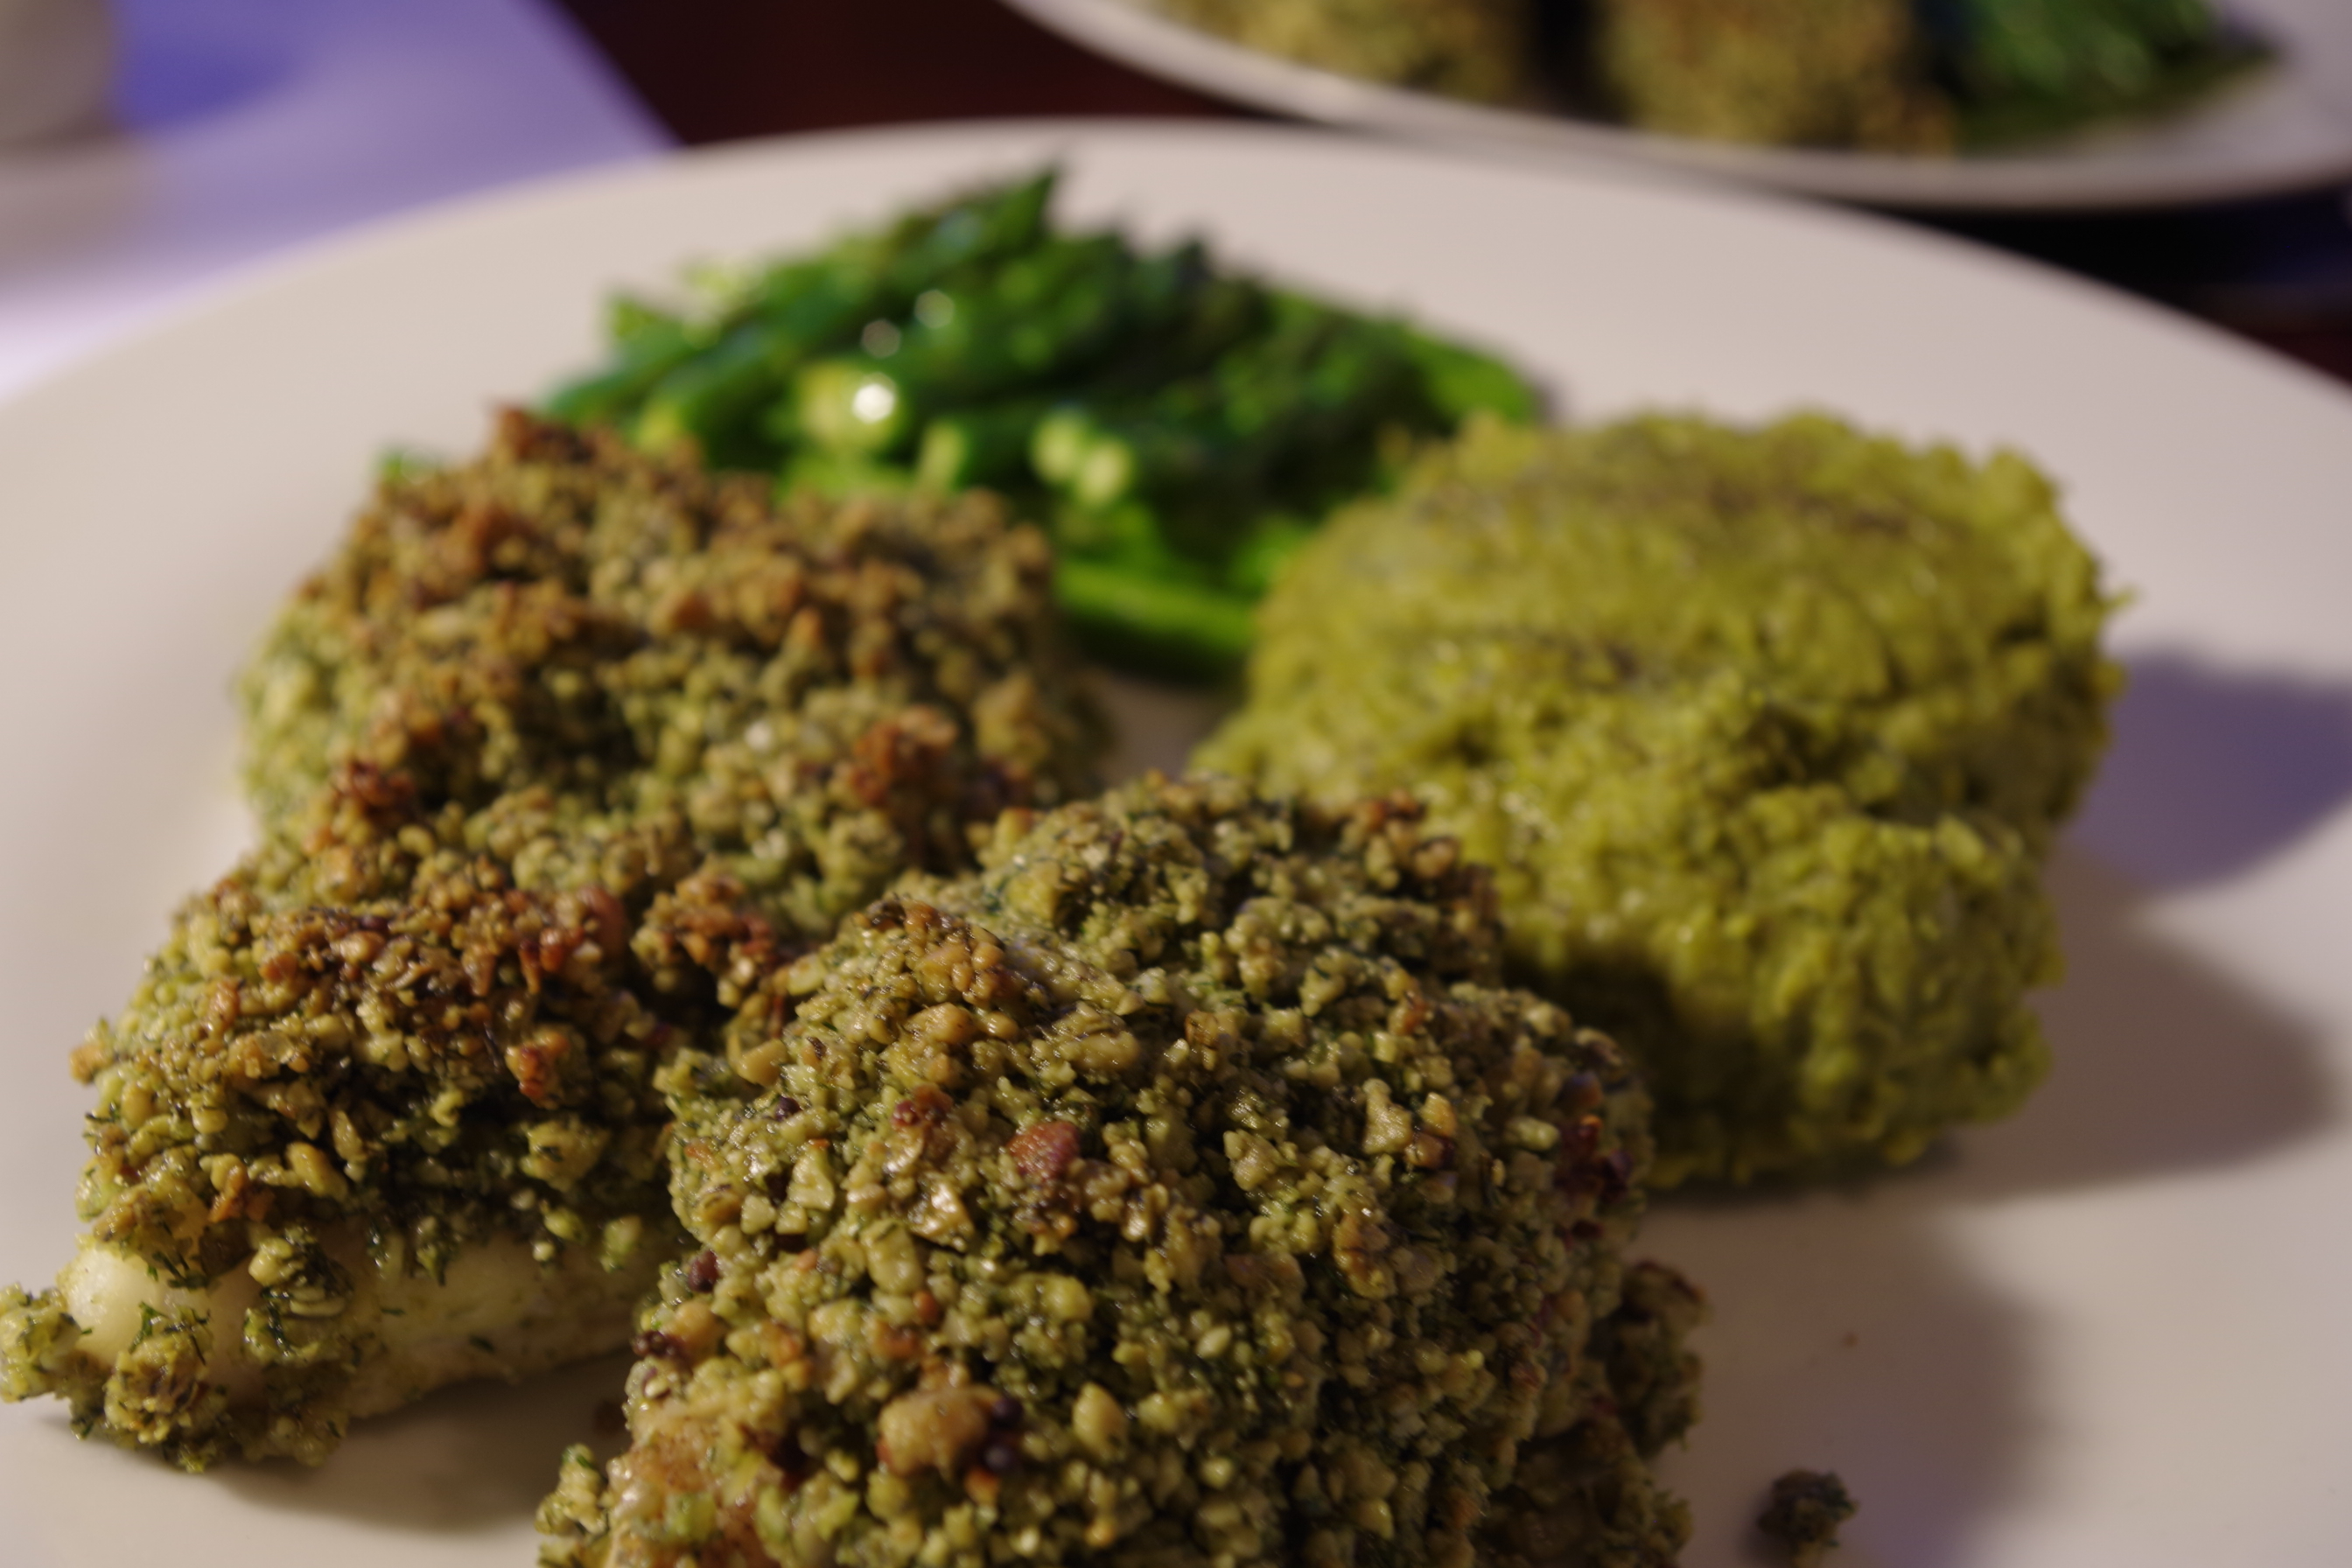
\includegraphics[width=\linewidth]{pestocrustfish.png}%
\end{figure*}

\section{Pumpkin seed and dill crusted cod}
\index{Fish!pumpkin seed \& dill}

An easy recipe from Nigel Slater. Serves 2.

\emph{2 fillets of boned, skinned, white fish\sidenote{Preferably cod. Slater warns against using an oily fish.}
\\75g pumpkin seeds
\\25g dill fronds and stems
\\2 tbsp olive oil
\\Mustard
}

\smallskip
\newpart{The crust:} 
\\Blend the dill, oil and pumpkin seedsin a food processor.
\\\newpart{Baking the fish:} 
\\Heat the oven to 180\celsius. Smear a thin layer of mustard on each piece of fish, then pack on the crust.
\\ Once hot, bake the fish for 12-15 minutes.

%%%%%%%%%%%%%%%%%%%%%%%%%%%%%%%%%%%%%%%%%
\chapter{Nana's curries}
%%%%%%%%%%%%%%%%%%%%%%%%%%%%%%%%%%%%%%%%%

\begin{figure*}[h]
  \includegraphics[width=\linewidth]{eggplantcurry.png}
\end{figure*}

\section{Nana's brinjal}
\index{Nana's!brinjal}
\index{Eggplant!Nana's brinjal}
\index{Vegetarian curries!Nana's brinjal}

Nana was known for creating the three greatest dishes in the culinary world (marrow bone mutton curry, Nana's rolls \& Nana's brinjol). The original eggplant dish required the vegetable to be fried. If you fry - the dish will be incredible, but it will soak up at least 250mls of oil. Hence the slightly more waistline friendly recipe below.

\smallskip
\emph{3-4 Brinjal (eggplant)
\\1 tbsp mustard seeds
\\a few heavy splashes of oil
\\3 onions, diced or sliced
\\1 tsp salt
\\1 chillies, finely diced
\\2 tsp tumeric
\\1 stem curry leaves
\\1 tin coconut milk}

\smallskip
Preheat the oven to 200\celsius 
\\Dice the brinjal and pour over the oil. Tip into an overproof tray and cook for 40 minutes, or till brown.
\\In a fry pan, fry the mustard seeds in a little oil.
\\Once the seeds start popping, add the onions, chilli, tumeric and curry leaves and fry till it starts to get brown.
\\Once browned, add the coconut milk, and cook on medium with the lid off for for 15 minutes.  
\\Add the aubergine back in, and serve.

%%%%%%%%%%%%%%%%%%%%%%%%%%%%%%%%%%%%%%%%%

\section{Curried vegetables}
\index{Vegetarian curries!Nana's}
\index{Nana's!Curried vegetables}

\emph{Any diced vegetables\sidenote{Potatoes, cauliflower, courgettes, carrots, etc.}
\\1/2 onions finely chopped
\\1 chilli sliced diagonally
\\1 stem curry leaves chopped
\\1 tsp mild indian curry powder
\\1/2 tsp turmeric
\\1 tsp garlic
\\1 tsp cumin seeds
\\1 ripe tomato, skinned and diced
\\1 tbsp water or stock
\\Salt
\\Oil for frying}

\smallskip
Gently fry onions, curry leaves, cumin seeds and chillies.\sidenote{Stir often during this step.}
\\Add potatoes and water and simmer.
\\Add other vegetables in order they need to cook.
\\Add tomatoes when almost cooked, the tomato forms the sauce.

%%%%%%%%%%%%%%%%%%%%%%%%%%%%%%%%%%%%%%%%%

\section{Nana's dahl}
\index{Nana's!dahl}
\index{Vegetarian curries!Nana's dahl}

This dish can be served a bit runny, or quite dry. I prefer it pretty dry, and with the dahl completely broken down, which can be achieved by cooking it for an extra hour or so.

\smallskip
\emph{1 1/2 cups red lentils
\\1/2 tsp turmeric
\\1 tsp salt
\\2 small green chillies, finely diced
\\5 tbsp ghee or butter
\\2 medium onions, finely chopped
\\1 tbsp fresh ginger, grated
\\2 large finely chopped tomatoes
\\1 tsp mustard seeds
\\1 tsp fennel seeds
\\1 tsp nigella seeds
\\1/2 tsp fenugreek seeds
\\4 curry leaves
\\2 small red chillies
\\2 cloves garlic, chopped}

\smallskip
Fry onions in 3 tbsp ghee. 
\\When beginning to brown, add ginger and tomatoes, cooking till the tomatoes are reduced.
\\Add dahl and 5 cups water and bring to the boil, with turmeric, salt and green chillies.
\\Simmer for 50 minutes, stirring and adding water if it gets thick enough to burn.
\\As the lentils begin to dissolve, fry the seeds, garlic and the whole red chillies till is begins to brown. 
\\Combine the spices and the dahl, and serve.\sidenote{Add one tin coconut milk to Nana's dahl. Stir in spinach, serve with half boiled eggs and coriander on top}

%%%%%%%%%%%%%%%%%%%%%%%%%%%%%%%%%%%%%%%%%

\section{Nana's chicken curry}
\index{Nana's!chicken curry}
\index{Meat curries!Nana's chicken}
\index{Chicken!Nana's curry}

A relatively easy curry. I like it with the skin removed, although you could try browning the chicken to make the skin more appealing.

\smallskip
\emph{1.25 kg chicken chopped
\\2 onions, finely chopped
\\2 chillies, chopped
\\10 curry leaves, chopped
\\2 tbsp Jaffna curry powder
\\1 tsp cinnamon, cloves, cardamon and salt
\\200ml coconut cream
\\1 clove garlic
\\2 tbsp chopped ginger
\\2 tsp fenugreek, cumin and fennel
\\Juice of one lemon
\\Salt
\\Oil}

\smallskip
Coat meat with curry powder and salt. 
\\Marinate for 24 hours in the fridge.
\\Gently fry onions, curry leaves, and chillies. When clear, add the spices and fry till brown.
\\Add the garlic and ginger and fry for 5 minutes.
\\Add meat and fry gently for 10 minutes.
\\Add the coconut cream and simmer gently for 20 minutes or until tender.
\\Add lemon juice just before serving.

%%%%%%%%%%%%%%%%%%%%%%%%%%%%%%%%%%%%%%%%%
\chapter{Meat curries}
%%%%%%%%%%%%%%%%%%%%%%%%%%%%%%%%%%%%%%%%%

\section{Lamb curry}
\index{Lamb!curry}
\index{Meat curries!Lamb}

Nana's lamb/mutton marrow bone curry is one of my favourite dishes. In Sri Lanka mutton usually means goat, but lamb is often substituted in New Zealand. While this isn't Nana's recipe - it's still worth seeking out marrow bones for the curry.

Jaffna curry powder is dark roasted, and while optional, without it the curry has a very different taste.

\smallskip
\emph{3 tbsp ghee or butter
\\1 kg bone in lamb, diced
\\1 tin tomatoes
\\200ml stock
\\2 chillies, chopped
\\10 curry leaves, chopped
\\1 tbsp Jaffna curry powder (optional)
\\2 tbsp fennel, cinnamon, cumin, coriander, fenugreek, pepper, all ground, cardamon
\\5cm ginger
\\2 red onions, diced
\\10 cloves garlic
\\1 big bunch coriander}

\smallskip
Pre-heat oven to 170\celsius.
\\Put everything from the chillies, to the garlic in a food processor. Add half the coriander, then blend.
\\In an oven proof dish, fry the paste in the butter till it goes brown.
\\Add the tomatoes and the stock, cover in foil, and place in the oven for 1.5 hours.
\\Remove the foil and return to the stove.
\\Add the lamb, and cook for 1.5 hours, with the lid off for about half that time.

%%%%%%%%%%%%%%%%%%%%%%%%%%%%%%%%%%%%%%%%%

\begin{figure*}[h]
  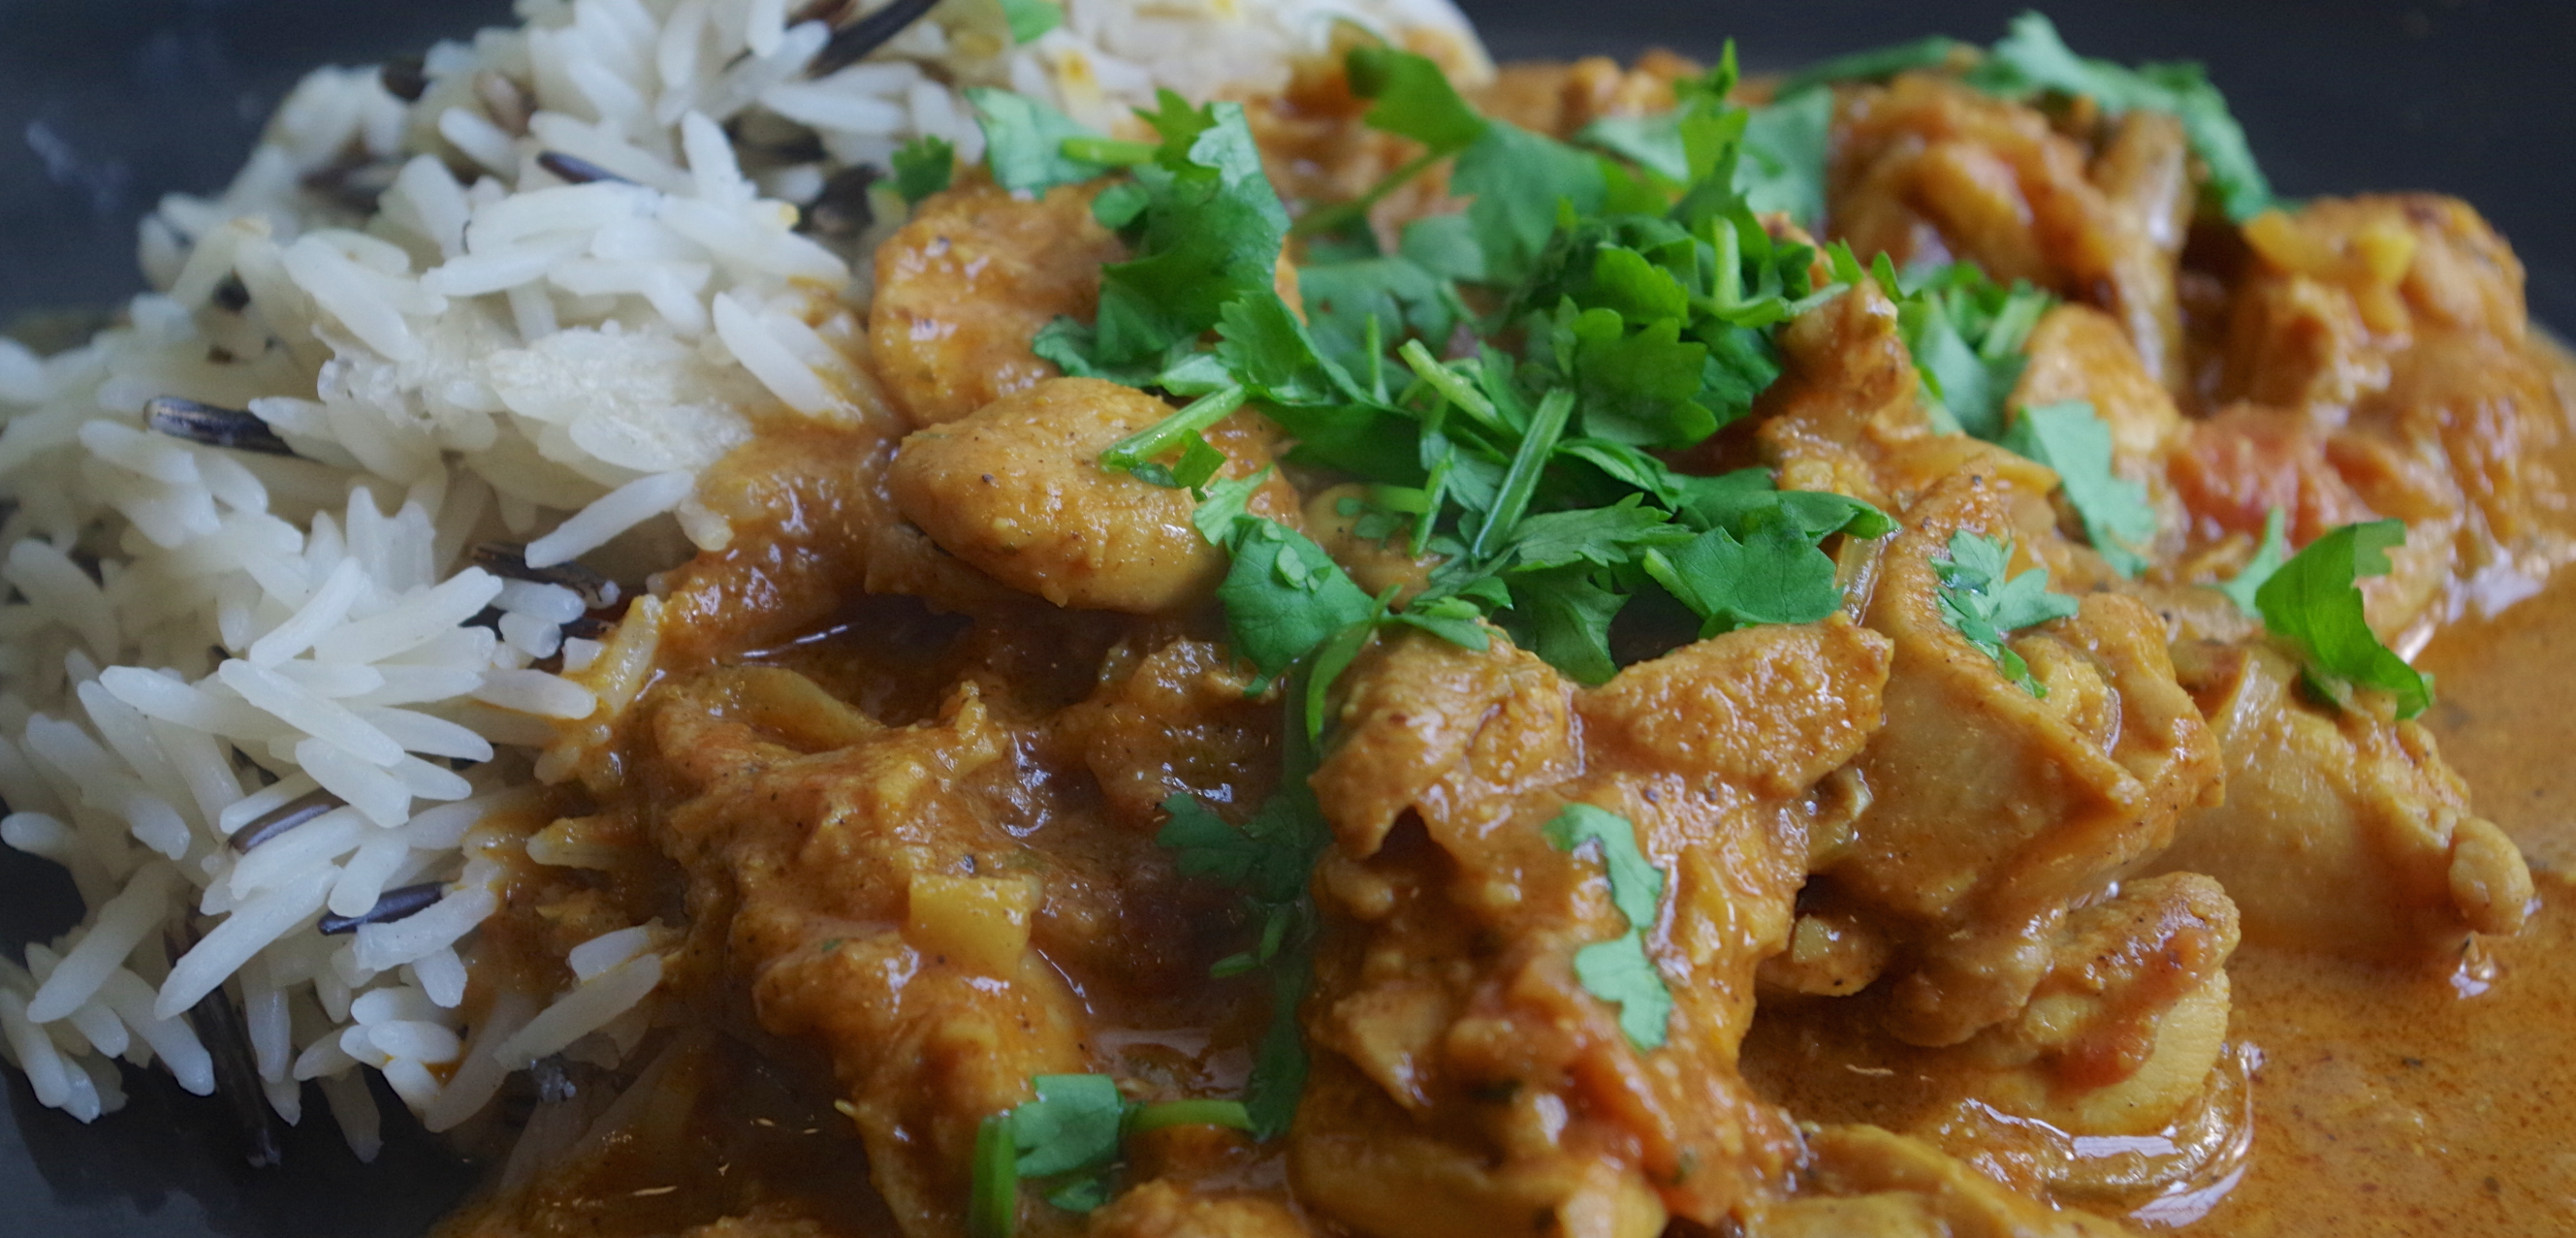
\includegraphics[width=\linewidth]{britcurry.png}%
\end{figure*}

\section{Chicken curry (Scottish style)}
\index{Chicken!curry}
\index{Meat curries!Chicken}

Similar to a chicken tikka masala, a Glaswegian curry, but without the sweetness or food colouring.

\smallskip
\newpart{For curry:}
\\\emph{4 skinless chicken thighs or breasts
\\2 onions
\\Thumb-sized piece of fresh ginger
\\1/2 bunch fresh coriander
\\1 fresh red chilli
\\1/2 tin of chopped tomatoes
\\400g tin coconut cream
\\Handful of flaked almonds, to serve
\\1 lemon, to serve}
\\\newpart{For spice paste:}
\\\emph{2 cloves of garlic
\\Thumb-sized piece of fresh ginger
\\1 teaspoon cumin seeds
\\1 teaspoon coriander seeds
\\1 teaspoon cayenne pepper
\\1 teaspoon sugar
\\2 teaspoons garam masala
\\1/2 teaspoon sea salt
\\2 tablespoons groundnut oil
\\2 tablespoons tomato puree
\\Small bunch of fresh coriander
\\1/2 tablespoon desiccated coconut
\\2 tablespoons ground almonds}

\smallskip
To make the curry paste, halve, deseed and roughly chop the chillies, then peel the garlic and ginger. 
\\Put a frying pan over a medium-high heat and add the cumin and coriander seeds. Lightly toast for a few minutes, or until golden brown and smelling delicious, then remove from the heat. 
\\Add the toasted spices to a pestle and mortar and grind until fine, or put them in a food processor and whiz to a powder. 
\\Once you've ground them, add the toasted spices to a food processor along with the remaining paste ingredients and whiz to a smooth paste, then put to one side.
\\Slice the chicken lengthways into 2cm strips. 
\\On a clean chopping board, peel, halve and finely slice the onions. Peel and finely slice the ginger, then pick the coriander leaves and put to one side, finely chopping the stalks along with the chilli.
\\Place a large casserole pan over a medium-high heat and add a couple of lugs of oil. Once hot, add the onions, chilli, ginger and coriander stalks, then cook for around 10 minutes, or until softened and lightly golden. 
\\Add the chicken and roughly 140g of the tikka masala paste, stirring well so everything is nicely coated. Season with salt and pepper, add the tomatoes and coconut milk (save the rest for another day), then bring everything to the boil.
\\Turn the heat down to medium-low, cover and simmer for 20 minutes, then take the lid off and cook for further 5 minutes, or until the meat is tender and the sauce has reduced, stirring occasionally. 
\\Divide the curry between bowls, sprinkle over the almonds and coriander leaves. Serve with fluffy rice, a dollop of yoghurt and lemon wedges for squeezing over.

%%%%%%%%%%%%%%%%%%%%%%%%%%%%%%%%%%%%%%%%%
\newpage

\section{Thai chicken curry}
\index{Meat curries!thai chicken}
\index{Chicken!thai curry}

\emph{2 tbsp oil
\\1 medium onion, sliced
\\2 cloves garlic, chopped
\\3 tbsp Thai red curry paste\sidenote{You can use red,green or even a penang curry paste here.}
\\3 kaffir lime leaves, chopped
\\500g minced chicken\sidenote{Or diced chicken or beef. If adding fish, add with the fish sauce and briefly simmer till cooked.}
\\1 cup coconut cream
\\1 cup chicken stock
\\1/2 cup crunchy peanut butter
\\2 tbsp fish sauce
\\1 tsp each salt and sugar
\\3 tbsp coriander, chopped
\\1-2 cups sliced or diced vegetables (zucchini, cauliflower, broccoli, carrots, beans, peas)
\\Spring onions or roasted peanuts}

\smallskip
Heat the oil, add the onion and garlic and cook.
\\Stir in the curry paste and lime leaves.
\\Add minced chicken, cook till meat is white.
\\Add coconut cream/stock and stir in peanut butter and cook for 8 minutes.
\\Add fish sauce, salt and sugar, serve when vegetables are cooked.

%%%%%%%%%%%%%%%%%%%%%%%%%%%%%%%%%%%%%%%%%
\chapter{Dessert}
%%%%%%%%%%%%%%%%%%%%%%%%%%%%%%%%%%%%%%%%%

\begin{figure*}[h]
  \includegraphics[width=\linewidth]{pumpkinpie.jpg}%
\end{figure*}

\section{Pumpkin pie}
\index{Dessert!pumpkin pie}
\index{Pie!pumpkin}
\index{Pumpkin!pie}

\emph{14 ounces chocolate wafers, finely ground
\\3/4 cup (1 1/2 sticks) unsalted butter, melted
\\1 pumpkin, roasted and blended.\sidenote{
You can also use 3 sweet potatoes, or 2 squashes. Just make sure to roast, not boil, and add a little water when you puree.}
\\1 (14 ounce) can sweetened condensed milk
\\1/2 lemon, juiced
\\5 tablespoons salted butter, melted
\\3 1/2 tablespoons light brown sugar
\\2 eggs
\\1 tablespoon vanilla extract
\\2 teaspoon ground cinnamon
\\1/2 teaspoon nutmeg
\\Sweetened whipped cream:
\\1 cup heavy cream
\\1/2 cup superfine sugar
\\1/2 teaspoon vanilla extract
\\Cadbury flake
}

\smallskip
Preheat oven to 170\celsius
\\\newpart{For crust:} 
\\In a large bowl mix together the chocolate wafer crumbs and melted butter until fully incorporated. Press the mixture into a pie dish or tart shell, pressing both evenly on the bottom and up the sides. Place onto a baking sheet and then into the refrigerator until ready to use.
\begin{marginfigure}%
  \includegraphics[width=\linewidth]{pumpkinpiesquare.png}
\end{marginfigure}
\newpart{For filling:} 
\\Place pumpkin puree in a bowl and add the remaining filling ingredients. Stir together until fully incorporated and no lumps remain. Pour the filling into the prepared crust and carefully set into the lowest rack of the oven. Bake for 55 to 70 minutes or until the filling has set, but is slightly loose in the middle.
\\Allow pie to cool completely, about 2 hours.
\\\newpart{For sweetened cream:} 
\\Pour cream, sugar and vanilla extract into a mixing bowl and beat together using an electric hand mixer until stiff peaks form.
\\Generously top pie with whipped cream and finish with the crumbled flake to serve.

%%%%%%%%%%%%%%%%%%%%%%%%%%%%%%%%%%%%%%%%%

\section{German mess}
\index{Dessert!German mess}

Apparently it's called "Raspberry Dream" in Germany. Really, it's an Eton Mess. The substitution of cream for the cheeses makes it taste a lot less creamy.

Ingredients for 6 portions:

\emph{200g meringue
\\500g frozen raspberries
\\500g mascarpone (or instead: 250g sour cream and 250g soft cheese)
\\250g quark
\\vanilla essence 
}

\smallskip
Mix mascarpone, quark, and vanilla.
\\Break meringue in pieces (not too small).
\\Fill mascarpone mix, raspberries and meringue in a bowl in layers.
\\Leave for 3-4 hours in the fridge.

\begin{figure*}[h]
  \includegraphics[width=\linewidth]{germanmess_banner.png}%
\end{figure*}


\backmatter

%\bibliography{sample-handout}
%\bibliographystyle{plainnat}


\printindex
\printindex[recipe][Recipe list]

\blankpage

\blankpage

\blankpage

\blankpage

\blankpage

\blankpage


\end{document}

